\chapter{Anomaly detection in multi-factor data} \label{sec:chapter_sgvaegan}

We propose a novel form of anomaly detection that considers several potential sources of anomalies. The approach is demonstrated on detection of semantic anomalies in image data, for which we have proposed the SGVAEGAN model. The model decomposes images into three independent components---the shape of an object and its foreground and background textures---and provides anomaly scores for each of those components separately. The source of anomality in the image can be identified by comparing the component scores. This novel concept  allows an explanation of the anomaly type in a completely unsupervised case. 
The overall anomaly score of an image is obtained by a weighted combination of the individual component scores. When a few labeled samples of anomalies are available, the model is able to learn the weights in the scores as a hyper-parameter. We have shown that this overall score is useful in the detection of anomalies in the semantic sense, where their anomalousness depends on the context in which they are evaluated. On classical anomaly detection benchmarks, the model was proven to outperform all baseline models. This was shown in a rigorous experimental study that covered the behavior of the model under a varying range of conditions.

section{Introduction}
\note{this was already covered in 1}
\note{
Anomaly detection~\cite{chandola2009anomaly, patcha2007overview} detects samples, which are in some sense different from those considered normal. The probabilistic definition assumes some probability distribution function $P,$ which is most of the time known only through a set of normal samples, and calls a sample anomalous if it lies in a region where $P$ has very low density. Anoumalous samples therefore raise a suspicion that they were generated by a different distribution than $P.$ Anomaly detection is important for many industries, where it is typically difficult to obtain representative training set to use supervised learning, for example network security~\cite{vanerio2017ensemble}, medical imagining~\cite{schleglFAnoGANFastUnsupervised2019}, video surveillance~\cite{zhou2019anomalynet}, and industrial process monitoring~\cite{mahmoudi2019layerwise, bai2020anomaly, choi2020gan}. In all these industries, users have some examples of anomalies, but there is a danger of a new type of anomaly to emerge, which contradicts the iid assumption of supervised learning.
 
Anomaly detection has been already extensively studied under many different names: outlier detection~\cite{knorr98algorithms,hodge2004survey}, novelty detection~\cite{pimentel2014review}, one-class classification~\cite{ruff2018deep} or out-of-distribution detection~\cite{liang2017enhancing}. All these approaches have in common is the assumption that only samples from the \textit{normal} class are available at training time. They model only the normal data and produce an \textit{anomaly score}, which is a measure of how much a sample deviates from the normality model. A recent large-scale study~\cite{vskvara2021comparison} has shown that classical methods~\cite{knorr98algorithms, scholkopf2001estimating, liu2008isolation, pevny2016loda} developed for tabular datasets of small dimension and number of samples work very well on them. But they do not work well on large high-dimensional datasets (typically containing image data), where modern methods built on top of deep neural networks~\cite{akcay2018ganomaly, perera2019ocgan, ruff2019deep, zavrtanik2021draem} work slightly better (we call these detectors deep anomaly detectors). 
}

The very same study also showed an inability of most deep anomaly detectors to detect \textit{semantic} anomalies. For example, an image (used in~\cite{vskvara2021comparison}) can be anomalous because it is blurred, or because it has a different object in the foreground (e.g. plane in the sky instead of a bird in the sky), or different background (e.g. the plane is on a runway, whereas it is usually on the sky). From the point of view of the above definition, they are all anomalies, but the user might be interested in anomalies of a certain type, or they might want the anomalies to be automatically sorted into different types. The detection of semantic anomalies has been previously studied under the name \emph{subspace} anomaly detection~\cite{raz2002semantic, kriegel2009outlier,rahmani2016randomized}. The idea, as the name suggests, is that the anomaly is not visible in the full input space, where it might be shadowed by noise, but only in the subspace. The subspace is most of the time "axis parallel" or defined in a linear transformation of the input space. 

It seems unlikely in practice that the subspace in which anomalies would be detectable would be aligned with the input space, or with its linear transformation. Contrary, independent components emerge after non-linear projections as shown in~\cite{burgess2018understanding, kim2018disentangling, esmaeili2019structuredhfvae, tschannen2018recent, bai2021contrastively, kim2019bayes, deecke2021transfer}, which motivates this work. We suggest to disentangle the input into independent factors, each providing an anomaly score. Ideally, a semantic anomaly would be then better detectable by one (few) of these scores rather than only a single complete score. 

This is the list of our contributions. 
\begin{itemize}
    \item We propose a new generative model for multi-factor image datasets based on contextual generative networks.
    \item We propose a multi-factor anomaly score: a weighted combination of  anomaly scores corresponding to individual factors of the latent space.
    \item We demonstrate that the proposed model is capable of detection of the most likely anomaly factor in the unsupervised setting, and quickly improves with very few labeled samples,
    \item We perform a large-scale study of the method on standard image benchmarks for anomaly detection together with a sensitivity analysis of the hyperparameter tuning on the number of known anomalies available for validation. With an increasing number of known anomalies, the problem is approaching a two-class problem, therefore, we also compare the method with a supervised classifier.
\end{itemize}

In the next section, we theoretically justify disentangled models and the proposed composition of their scores. In Sec.~\ref{sec:model}, the model used in experiments is described together with details of its construction, training, and evaluation. Sect.~\ref{sec:related_work} discusses the related work, and in the experimental Sec.~\ref{sec:experiments}, the proposed model is extensively compared to baselines on several image benchmarks.

\section{Decomposing the anomaly score} 
\label{sec:theory}
Variational autoencoder (VAE)~\cite{kingma2013vae} fits a generative model with data $x \in \mathbb{R}^n$
\begin{align}
p(x) & = \int p_{\theta}(x \vert z)p(z)dz & p_{\theta}(x\vert z) & =\mathcal{N}(x;g_{\theta}(z),\sigma^{2} \mathbf{I}),\label{eq:vae}
\end{align}
where the prior on the latent $k$-dimensional variable $z$ is either fixed $p(z)=\mathcal{N}(0,\mathbf{I})$, or further parametrized $p_{\theta}(z)$ as in~\cite{tomczak2017vae}. Distribution $p_{\theta}(x\vert z)$ is frequently called \emph{decoder} with $g_{\theta}(z)$ being realized by a neural network parametrizing the mean of the normal distribution. To fit the model, VAE introduces an \emph{encoder}, which is a conditional probability distribution $q_{\phi}(z\vert x)$ parametrized similarly to the decoder as $q_{\phi}(z\vert x)=\mathcal{N}(z;\mu_{\phi}(x),\text{diag}(\sigma_{\phi}(x)))$ with $mu_{\phi}(x), \sigma_{\phi}(x)$ being neural networks. During training, parameters $(\theta,\phi)$ of both neural networks are optimized to maximize the evidence lower bound (ELBO) on given training samples.

Estimated parameters $(\theta,\phi)$ uniquely define marginal likelihood in \eqref{eq:vae}, but since the expression contains a complex integral, in practice it is crudely approximated by the reconstruction error as 
\begin{equation}
p(x)\approx\int p_{\theta}(x\vert z)\delta(z-\mu_{\phi}(x))dz\ \propto\ \exp\left(-\vert x-g_{\theta}(\mu{\phi}(x))\vert ^{2}\right), \label{eq:px-vita}
\end{equation}
where $\propto$ denotes equality up to a multiplicative constant. Notice that in this expression, the integration over $z$ is replaced by an evaluation of the likelihood at the "most probable" point given by the encoder $q_{\phi}(z\vert x).$

\subsection{Orthogonal generative model}
The above generative model~\eqref{eq:vae} can be rewritten as $x=g_{\theta}(z)+e$ where $e$ is (usually isotropic) Gaussian noise. This formulation  emphasizes the need for marginalization since $g_{\theta}(z)$ is a random variable of dimension $k,$ and noise $e$ is a random variable of dimension $n,$ which is the same as the data. Equation~\eqref{eq:vae} therefore marginalizes away random variables corresponding to latent $z.$ An alternative formulation~\cite{pidhorskyi2018generative, vsmidl2019anomaly} assumes orthogonal decomposition of the noise as
\begin{align}
x&=g_{\theta}(z)+e & \rightarrow & &x=g_{\theta}(z')+e^{\bot},
\end{align}
where $z'$ is a point in the latent space, and $e^{\bot}$ is the observation noise that lies in the normal space perpendicular to the manifold defined by the decoder $g_{\theta}(z)$. Denoting $x'=g_{\theta}(z'),$ any point $x$ can be decomposed  into 
\begin{align*}
x & =x'+e^{\bot},
\end{align*}
where $x'$ lies on a $k$-dimensional manifold, and $e^{\bot}$ in its normal space (of $n-k$ dimensions). 

Due to the (local) orthogonality, $x'$ and $e^{\bot}$ can be considered independent and therefore probability distribution $p(x)$ to be well approximated as $p'(x)p(e^{\bot})$. Since the probability of $p'(x)$ is given by the change of coordinate formula from $p_{z}(z)$, and $p(e^{\bot})\approx p(e)$, for the likelihood $p(x)$ now holds
\begin{align}
p(x)\approx p'(x)p(e)=p_{z}(g_{\theta}^{-1}(x))\left\vert \frac{\partial g_{\theta}^{-1}(x)}{\partial x}\right\vert p(e).\label{eq:pxjacodeco}
\end{align}
A gaussian noise model might be assumed, e.g. $p(e) = \mathcal{N}(x-x',\sigma^{2}\mathbf{I})$. Note that the assignment $p(e^{\bot})=p(e)$ is correct up to a normalizing constant if the $z'$ point is correctly estimated (more on this in Sec.~\ref{sec:sgvaegan}).

In practice, an anomaly score $s(x) = - \log p(x)$ is computed as
\begin{align}
s(x) & = - \log p(e) -\log p_{z}(z)-\log\left\vert \frac{\partial g_{\theta}^{-1}(x)}{\partial x}\right\vert ,\label{eq:jacodeco}
\end{align}
which is essentially the reconstruction error with additional terms. We will use $s$ to denote various unnormalized anomaly scores throughout this text.

\subsection{Anomaly in the latent space}
Let's now observe how the above generative model changes when we assume the distribution on latent $z$ to be multi-modal conditioned by hidden label $y$
\begin{equation} \label{eq:pzy}
p(z\vert y)=p_{n}(z)^{y}p_{a}(z)^{1-y},y\in[0,1],
\end{equation}
where $y=1$ for normal data, $y=0$ for anomalies, and $p_n(z),p_a(z)$ are the latent distributions of normal and anomalous data, respectively. Then from~\eqref{eq:jacodeco} we have
\begin{align*}
s(x \vert y) & = - \log p(e) -y\log p_{n}(z) - \log\left\vert \frac{\partial g_{\theta}^{-1}(x)}{\partial x}\right\vert -(1-y)\log p_{a}(z),
\end{align*}
Since $y$ is usually unknown, we will integrate it away by expectation over all possible $y$, 
\begin{align}
\mathbb{E}_{p(y)} \left[  s(x \vert y) \right]  = &  - \log p(e) - \log\left\vert \frac{\partial g_{\theta}^{-1}(x)}{\partial x}\right\vert \nonumber \\ 
 & - \int_{\mathcal{Y}} y\log p_{n}(z) p(y) dy - \int_{\mathcal{Y}} (1-y)\log p_{a}(z) p(y) dy \nonumber \\
   \propto & - \log p(e) - \log\left\vert \frac{\partial g_{\theta}^{-1}(x)}{\partial x}\right\vert  - \alpha\log p_{n}(z) = s(x). \label{eq:jacodeco2}
\end{align}
where we assume $\mathbb{E}_{p(y)} \left[  y \right] =\alpha$, and $p_{a}(z)\propto1$ (because the probability of an anomaly is assumed to be the same everywhere). 


Now consider a \emph{disentagled} model, where data are generated from multiple independent latent spaces, $z_{i}=z_{1},\ldots,z_{l}$, 
\begin{equation} \label{eq:multilatent}
x=f(z_{1},\ldots,z_{l})+e,
\end{equation}
where each of the latents has distribution $p(z_{i})=\mathcal{N}(0,\mathbf{I})$. Each of the latent spaces can be a potential source of various types of anomalies, with hidden labels  $y=(y_{1},\ldots,y_{l})   $. Therefore, instead of~\eqref{eq:pzy},  we have
\begin{equation} 
p(z\vert y)= \prod_{i=1}^l p_{n_i}(z_i)^{y_i}p_{a_i}(z_i)^{1-y_i},y_i\in[0,1].
\end{equation}
Repeating derivation of (\ref{eq:jacodeco2}) for multiple latent variables, the anomaly score becomes
\begin{align} \label{eq:alphadeco}
s(x) & = - \log p(e) - \log\left\vert \frac{\partial g_{\theta}^{-1}(x)}{\partial x}\right\vert  -  \sum_{i=1}^{l}\alpha_{i}\log p_{n_{i}}(z_{i}),
\end{align}
where $\alpha_{i}$ is denoting probability that the latent variable of the $i$th factor is generated from the normal class. In this work, we assume that $\alpha_i$ is not known during training but has to be estimated in the validation stage from examples of anomalous samples.\footnote{Based on the  industrial experience of authors, this assumption is safe, i.e. there are usually examples of anomalies, though their diversity might be low.}

The interpretation of the values of $\alpha_i$ will be important later, in Sec.~\ref{sec:model}, where we construct the latent spaces in order to give them a specific meaning, and in Sec.~\ref{sec:anomaly_detection}, where we describe their fitting. Fitting values of all $\alpha_i$ on a set of labeled data is equal to estimating the mean of $p(y_i)$ for the given data. This can be interpreted as estimating how likely it is for an anomaly to appear in the $i$-th latent in the context of the current dataset. 

In contrast, for a single data sample, we are more interested in the actual values of $y_i$, which are binary and which determine whether the sample is anomalous in the context of the latent space $i$. Their estimation is equal to the estimation of the distributions $p(y_i \vert x)$ and will be discussed in Sec.~\ref{sec:anomaly_factor_identification}. 

\section{Shape-guided decomposition} \label{sec:model}
\begin{figure}[ht!]
    \centering
    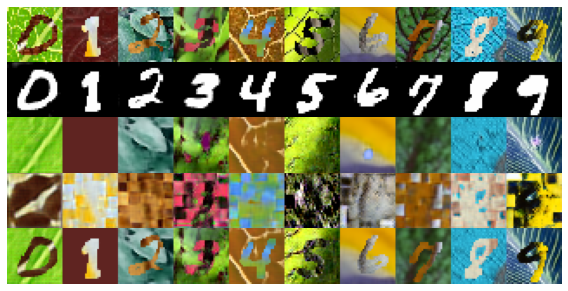
\includegraphics[width=\textwidth]{data/chapter_sgvaegan/wmnist_grid.png}
    \caption{Examples of decomposition on the wildlife MNIST dataset by the SGVAEGAN model. The first row contains the input samples, below that are the decoded masks, backgrounds, foregrounds, and finally the whole reconstructions. The model can learn appropriate masks in an unsupervised fashion.}
    \label{fig:wmnist_grid}
\end{figure}

We demonstrate the advantage of disentanglement in detecting anomalies on image data, because (i) the disentanglement has been researched mostly in this domain~\cite{kim2018disentangling, kim2019bayes, choi2020discond}, (ii) most public datasets are in this domain, (iii) the anomaly detection community is the most active in this field.

We assume an image $x$ to be composed of three main components: a mask (shape of the object), a background texture, and a foreground texture (the object). The mask together with the foreground texture defines the semantic meaning of the object, as it is what defines the class of the image in datasets. According to the above assumptions, each component (mask, background texture, and foreground texture) is generated from an independent variable. Therefore, for the latent distribution $p(z)$ it holds that
\begin{equation} \label{eq:latent_decomposition}
     p(z) = p_{z_{m}}(z_{m})p_{z_{f}}(z_{f})p_{z_b}(z_{b}),
\end{equation}
where subscripts $m,f,b$ denote the mask, foreground, and background latent variable, respectively. 
A representative example of a dataset where each image is composed of three independent components is the wildlife MNIST dataset~\cite{sauer2021counterfactual}. It is constructed using masks from MNIST~\cite{lecun2010mnist} combined with foreground and background textures from~\cite{cimpoi2014describing} (see more details on its construction in Sec.~\ref{sec:datasets}). For examples from individual classes see the top row of Fig.~\ref{fig:wmnist_grid}. 

The independent decomposition~\eqref{eq:latent_decomposition} is akin to~\eqref{eq:multilatent}, but here we ascribe meaning to the individual latent spaces. This means that the model built on top of the assumption~\eqref{eq:latent_decomposition} has an inductive bias, which enables the unsupervised disentangled representation of the individual components of an image. The independency is further reinforced by the fact that the parts of the model responsible for the representation of the components will not share parameters. Also, since we want to apriori ascribe specific meaning to the disentangled latents, we cannot use automatic disentanglement of individual dimensions as is the case in literature~\cite{burgess2018understanding, kim2019bayes, deecke2021transfer}, since there, the meaning can be given to the individual dimensions only using a manual post-hoc analysis with labeled data. Another argument against disentanglement on the level of individual latent dimensions is the fact that eventually the model is used to compute anomaly score~\eqref{eq:alphadeco}, and using too many $\alpha_i$ values would likely lead to overfitting, since labeled anomalies are scarce.

In this chapter, the structure of the proposed generative model with independent latent spaces and its training procedure are described first. Then, we combine the model with the anomaly score derived in the previous chapter in order to be able to detect and describe semantic anomalies.

\subsection{Shape-guided VAEGAN model} \label{sec:sgvaegan}
\begin{figure}[ht]
    \centering
       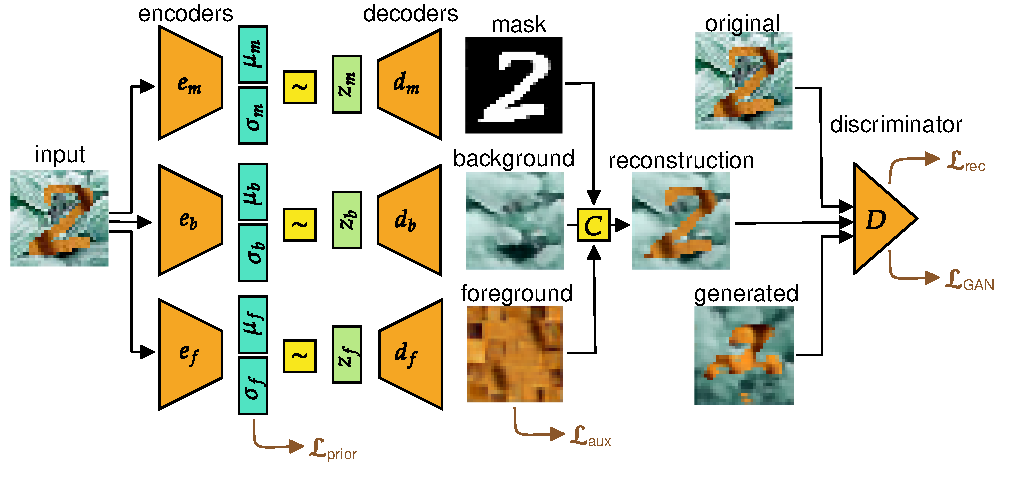
\includegraphics[width=\textwidth]{data/chapter_sgvaegan/sgvaegan_losses.pdf}
    \caption{Schema of the proposed model. Convolutional blocks are denoted in orange, fully connected in cyan, and intermediate representations in green. The yellow squares represent special operations - $c$ is the composition~\eqref{eq:composition} and the reparametrization trick is denoted by $\sim$. The generated sample is obtained by feeding samples from priors $\mathcal{N}(0,\mathbf{I})$ to the decoders.}
    \label{fig:sgvaegan_schema}
\end{figure}

The model disentangling the input image into its three components is our synthesis of a VAEGAN~\cite{larsen2016autoencoding} and Counterfactual generative networks (CGN)~\cite{sauer2021counterfactual}.\footnote{Counterfactual generative networks~\cite{sauer2021counterfactual} were selected because based on our preliminary experiments, the result offered superior disentanglement likely due to highly inductive bias.} Building blocks of this model, further denoted SGVAEGAN, are outlined in Fig.~\ref{fig:sgvaegan_schema}. The model uses three separate independent autoencoders for three components of an image, a block combining them to the reconstructed image, and a discriminator for a tighter fit. We emphasize that it is this strict separation of autoencoders that motivates the desired disentanglement.

Autoencoders responsible for individual components are vanilla VAE consisting of an encoder
\begin{equation} \label{eq:encoder}
    q_{i}(z_i \vert x, \theta) = \mathcal{N} \left(z_i; \mu_i(x\vert\theta), \text{diag}(\sigma_i(x\vert\theta)) \right),\quad i \in \lbrace m, f, b \rbrace,
\end{equation}
 and a decoder 
\begin{equation} \label{eq:decoder}
    x_i = g_i (z_i\vert\theta),\quad i \in \lbrace m, f, b \rbrace.
\end{equation}
Latent variables $z_i$ are sampled through the usual reparametrization trick~\cite{kingma2013vae} from a normal distribution~\eqref{eq:encoder} with a diagonal covariance matrix.

All three autoencoders output a tensor of the size of the input image, $x_m,$ $x_f,$ and $x_b,$ which are composed by a compositor $c(x_m,x_f,x_b)$ as
\begin{equation}
    x' = c(x_m,x_f,x_b) = x_m \odot x_f + (\mathbf{1} - x_m) \odot x_b, \label{eq:composition}
\end{equation}
where $\odot$ denotes Hadamard (element-wise) product and $\mathbf{1}$ is a matrix of ones with the same dimension as $x_m.$ The elements of the mask $x_m$ lie in the interval $[0,1]$ and the training procedure ensures that they are pushed to the extremes of the closed interval, such that elements with nonzero values represent the pixels that contain the most prominent object in the image. 

The \emph{loss function} optimized during training consists of a reconstruction error, GAN-loss, regularization of the latent space, and auxiliary part, 
\begin{equation}
    \mathcal{L} = \lambda_{\text{rec}}\mathcal{L}_{\text{rec}} + \mathcal{L}_{\text{GAN}} +  \mathcal{L}_{\text{prior}} + \mathcal{L}_{\text{aux}}.
    \label{eq:loss}
\end{equation}
Their contributions are controlled by a scalar weight $\lambda_{\text{rec}}$ and by weights contained in $\mathcal{L}_{\text{aux}}.$ The first three parts in Eq.~\eqref{eq:loss} are adopted from VAEGAN while the last part from CGN. The rest of this section describes them in detail.

The \emph{reconstruction loss} uses a "feature-matching" construction~\cite{salimans2016fmgan}, which was chosen because of its good results in~\cite{vskvara2021comparison}. It generalizes standard reconstruction loss by comparing $x$ and $x'$ at a certain depth of the discriminator  as
\begin{equation} \label{eq:recloss}
     \mathcal{L}_{\text{rec}} = L_{\text{fm}}(x,k) =\vert \vert d_k(x) - d_{k}(x{'}) \vert \vert_2,
\end{equation} 
where $d_k(x)$ is the intermediate representation of $x$ at the $k$-th layer of the discriminator. When $k=0$, the loss coincides with the classical log-likehood $-\mathbb{E}_{q(z \vert x)}[\log p(x \vert z)]$ for VAE with gaussian output distribution. In the experiments in Sec.~\ref{sec:experiments}, $k$ is treated as a hyperparameter subjected to tuning.\footnote{Based on our experimental results, we cannot recommend a single good value, as values selected on the validation set ranged from 0 to 7.} The authors of the VAEGAN model claim that incorporating the discriminator for image reconstruction leads to better overall reconstruction/generation quality as it pushes the model to be able to abstract beyond the capabilities of pixel-wise reconstruction loss~\eqref{eq:recloss}.

The \emph{GAN loss} $\mathcal{L}_{\text{GAN}}$ was adopted from the VAEGAN model. It optimizes the discriminator $d$ and the decoders $g_{m,\theta},$ $g_{f,\theta},$ and $g_{b,\theta},$ of the model via
\begin{equation} \label{eq:ganloss}
    \mathcal{L}_{\text{GAN}} = - \log d(x) - \log (1 - d(x')) - \log (1-d(\tilde{x})),
\end{equation}
where $\tilde{x}$ is a sample that was generated by decoding latent codes $\tilde{z}_m,$ $\tilde{z}_f,$ and $\tilde{z}_b$ sampled from $\mathcal{N}(0,\textbf{I})$ instead from the learned latents~\eqref{eq:encoder} and composing them via~\eqref{eq:composition}. The discriminator outputs a scalar in the range $[0,1]$, where a higher value is meant to be assigned to a sample coming from the training dataset and a lower to the reconstructed/generated image. This is achieved by minimizing the loss~\eqref{eq:ganloss} with respect to the discriminator parameters and maximizing it with respect to the decoders' parameters. This is similar to discriminator/generator training in a classical GAN~\cite{goodfellow2014gan}.

The \emph{regularization} of the latent space is done by the usual KL divergence~\cite{kingma2013vae} between the learned latent distribution $q_{\phi} (z \vert x)$ and the prior $p(z)$ as
\begin{equation} \label{eq:kldloss}
    \mathcal{L}_{\text{prior}} = D_\text{KL} (q_{\phi} (z \vert x) \vert \vert p(z)) = \sum_{i \in \lbrace m, f, b \rbrace} D_\text{KL} (q_{i,\phi} (z_i \vert \vert x) \vert p(z_i)),
\end{equation} 
where the sum is possible because it is assumed $z_i$ to be independent. Furthermore, since it is assumed $p(z_i) = \mathcal{N}(0,\mathbf{I})$, $\mathcal{L}_{\text{prior}}$ can be computed analytically~\cite{kingma2013vae}.

The \emph{auxiliary loss}, adopted from~\cite{sauer2021counterfactual}, is a weighted combination of three parts
\begin{equation} \label{eq:auxloss}
    \mathcal{L}_{\text{aux}} = \lambda_{\text{bin}}\mathcal{L}_{\text{bin}}(x_m) + \lambda_{\text{mask}}\mathcal{L}_{\text{mask}}(x_m) + \lambda_{\text{text}}\mathcal{L}_{\text{text}}(x_m,x_f,x).
\end{equation} 
The texture loss $\mathcal{L}_{\text{text}}(x_m,x_f,x)$ ensures that the parts of the network assigned to reconstruct the background and foreground are not switched and that no shape information is stored in the mask. It is computed in the following way: 36 patches are sampled from the image $x$ in regions where the mask $x_m$ is nonzero. These are then composed together to form a tensor $x_g$ that is as large as the image. Then, a perceptual loss~\cite{johnson2016perceptual} between $x_g$ and $x_f$ is minimized. The perceptual loss is computed as the L1 distance between the activation maps of $x_f$ and $x_g$ in the first four convolutional layers of a VGG16~\cite{simonyan2014very} network.

The term $\mathcal{L}_{\text{bin}}$ forces elements of the mask to be close to either 0 or 1. The objective to be minimized is
\begin{equation}
    \mathcal{L}_{\text{bin}}(x_m) = - \frac{1}{N} \sum_{i}^N x_{m,i} \log_2(x_{m,i}) + (1-x_{m,i}) \log_2(1 - x_{m,i}),
\end{equation}
where the index $i$ goes over all the elements of the tensor $x_m$ and $N$ is the number of its elements.

 Finally, $\mathcal{L}_{\text{mask}}$ prevents degeneration of the mask to be all zeroes or all ones, which would lead to failure in the identification of background / foreground. This is achieved by computing
  \begin{equation}
    \mathcal{L}_{\text{mask}}(x_m) = \left[ \max \left( 0, \tau - \frac{1}{N} \sum_{i}^N x_{m,i} \right) + \max \left( 0, \frac{1}{N} \sum_{i}^N x_{m,i} -\tau  \right) \right]
\end{equation}
where $\tau \in [0,1]$ is a parameter that forces the mask to occupy a total area of the image that is in the interval $[\tau, 1-\tau]$. 

The complete training procedure of the SGVAEGAN model is described in detail in Alg.~\ref{alg:training}.

\begin{algorithm}
\caption{Training of the SGVAEGAN model. The budget is either a time limit or a fixed maximum number of iterations. Capital letters denote a batched variable.}\label{alg:training}
\begin{algorithmic}[1]
\Require Training set, $(\phi, \theta, \varphi) = $ (encoder, decoder, discriminator) parameters.
\State $(\phi, \theta, \varphi)  \leftarrow $ initialize parameters
\While{$(\phi, \theta, \varphi)$ not converged or budget exhausted}
\State $X \leftarrow $ batch of $L$ samples from the dataset
\State // Computation of prior, reconstruction and auxilliary losses
\State $(Z_m, Z_f, Z_b) \leftarrow $ encodings of $X$
\State $\mathcal{L}_{\text{prior}} \leftarrow \sum_{i \in \lbrace m, f, b \rbrace} D_\text{KL} (q_{i,\phi} (Z_i \vert \vert X) \vert p(Z_i))$  
\State $(X_m,X_f,X_b) \leftarrow (g_{m, \theta}(Z_m), g_{f, \theta}(Z_f), g_{b, \theta}(Z_b))$ 
\State $X' \leftarrow c(X_m,X_f,X_b)$
\State $\mathcal{L}_{\text{rec}} \leftarrow \vert \vert d_l(X) - d_l(X') \vert \vert_2$
\State $\mathcal{L}_{\text{aux}} \leftarrow \lambda_{\text{bin}}\mathcal{L}_{\text{bin}}(M) + \lambda_{\text{mask}}\mathcal{L}_{\text{mask}}(M) + \lambda_{\text{text}}\mathcal{L}_{\text{text}}(M,F,X).$
\State // Adversarial loss 
\State $(\tilde{Z}_m, \tilde{Z}_f, \tilde{Z}_b) \leftarrow $ samples from the prior
\State $(\tilde{X}_m,\tilde{X}_f,\tilde{X}_b) \leftarrow (g_{m, \theta}(\tilde{Z}_m), g_{f, \theta}(\tilde{Z}_f), g_{b, \theta}(\tilde{Z}_b))$ 
\State $\tilde{X} \leftarrow C(\tilde{X}_m,\tilde{X}_f,\tilde{X}_b)$
\State $\mathcal{L}_{\text{GAN}} \leftarrow - \log d(X) - \log (1 - d(X')) - \log (1-d(\tilde{X}))$
\State // Update of the parameters
\State $\phi \stackrel{+}\leftarrow -\nabla_{\phi} (\lambda_{\text{rec}} \mathcal{L}_{\text{rec}} + \mathcal{L}_{\text{aux}} + \mathcal{L}_{\text{prior}})$
\State $\theta \stackrel{+}\leftarrow -\nabla_{\theta} (\lambda_{\text{rec}} \mathcal{L}_{\text{rec}} + \mathcal{L}_{\text{aux}} - \mathcal{L}_{\text{GAN}})$
\State $\varphi \stackrel{+}\leftarrow -\nabla_{\varphi} \mathcal{L}_{\text{GAN}}$
\EndWhile
\end{algorithmic}

\end{algorithm}

\subsection{Detecting anomalies with SGVAEGAN} \label{sec:anomaly_detection}

\begin{figure}[ht!]
    \centering
        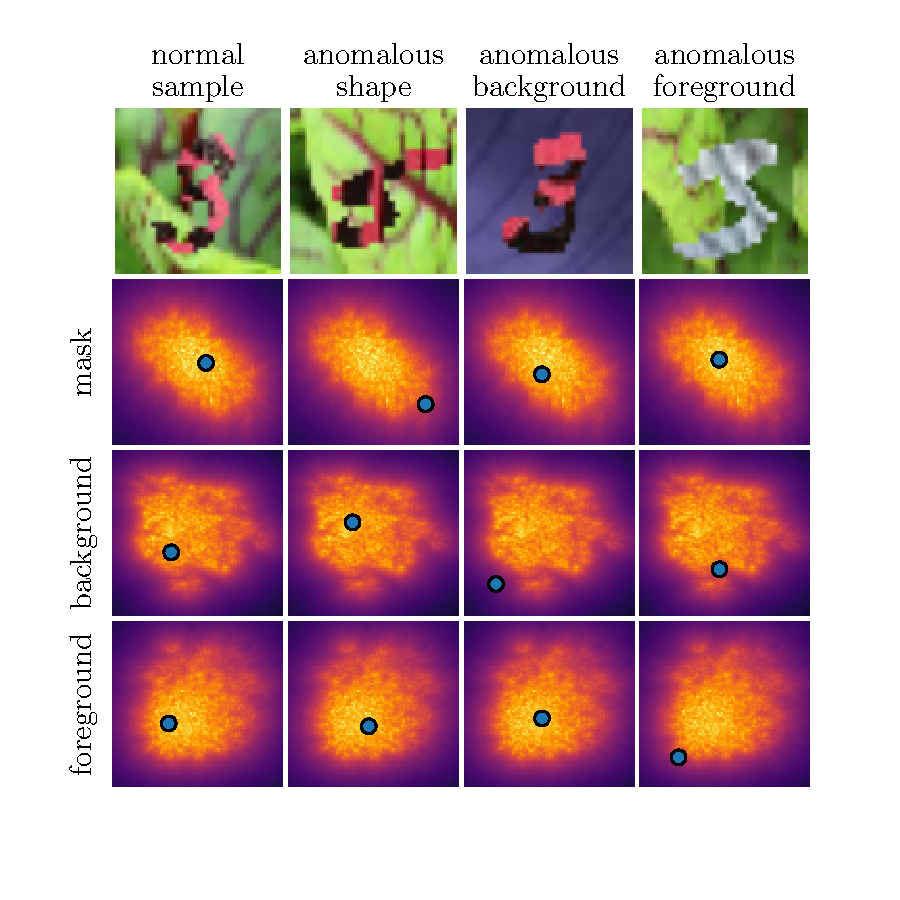
\includegraphics[width=0.95\textwidth]{data/chapter_sgvaegan/latent_decomposition_example.pdf}
    \caption{Position of different images encoded to individual latent spaces using SGVAEGAN model with two-dimensional latent spaces. The training set consisted of images with factors fixed to those of the digit in the first column. Also depicted are the densities of encodings of normal (training) data, estimated by a kNN detector~\eqref{eq:knnscore}.}
    \label{fig:latent_decomposition_example}
\end{figure}

If the SGVAEGAN is trained well, particularly if decomposition into latent spaces is (at least approximately) right, different types of anomalies should be in low-density regions of different latent spaces, as is illustrated in Fig.~\ref{fig:latent_decomposition_example} on the wildlife MNIST dataset, where we see that anomalous shape, background texture, and foreground texture is anomalous in the corresponding latent space. We can use the score~\eqref{eq:alphadeco} and assign $p_{n_i}(z_i) = p_{z_i}(z_i), i \in \lbrace m,f,b \rbrace$, since the model is trained on normal data. Then we have
\begin{equation}
s(x) = - \log p(e)  - \log\left\vert \frac{\partial g^{-1}(x)}{\partial x}\right\vert -  \sum_{i\in\{m,f,b\}}\alpha_{i}\log p_{z_{i}}(z_{i}),	
\label{eq:scorewithx}
\end{equation}
where
\begin{equation}
g(z) = g(z_m, z_f, z_b) = g_m(z_m) \odot g_f(z_f) + (1 - g_m(z_m)) \odot g_b(z_b).
\end{equation}
Following derivations in~\cite{vsmidl2019anomaly}, we use the fact that $\frac{\partial g^{-1}(x)}{\partial x} = \left( \frac{\partial g(z)}{\partial z} \right) ^{-1}$, and assume the independency of latent spaces $z_m, z_f, z_b$, then Eq.~\eqref{eq:scorewithx} can be rewritten to 
\begin{align} \label{eq:scorejacodeco}	
s(x) & = - \log p(e)  + \sum_{i\in\{m,f,b\}} \log\left\vert \frac{\partial g(z_m, z_f, z_b)}{\partial z_i}\right\vert -  \sum_{i\in\{m,f,b\}} \alpha_{i}\log p_{z_{i}}(z_{i}) \\
& = - \log p(e)  + J_d(x) -  \sum_{i\in\{m,f,b\}} \alpha_{i}\log p_{z_{i}}(z_{i}),
\end{align}
where $J_d(x)$ denotes the sum of jacobian terms functionally dependent on the input image $x$ through~\eqref{eq:encoder}. A reader recognizes that $\frac{\partial g(z_m, z_f, z_b)}{\partial z_i}$ in~\eqref{eq:scorejacodeco} is not square, hence its determinant is zero. Ref.~\cite{vsmidl2019anomaly} suggest estimating the determinant from a diagonal matrix after SVD decomposition, which is valid if one assumes the orthogonality of the data and noise (see~Alg.~\ref{alg:jdx}).

% use this such that procedure starts with small letters
\algrenewcommand\textproc{} 
\begin{algorithm}
\caption{Calculation of $J_d(x)$}\label{alg:jdx}
\begin{algorithmic}[1]
\Require image $x$, encoder means $\mu_{i,\phi}$, decoders $g_{i,\theta}$, $i \in \lbrace m, b, f \rbrace$
\State $\left(z_m, z_b, z_f \right) \leftarrow \left(\mu_{m,\phi}(x), \mu_{b,\phi}(x), \mu_{f,\phi}(x) \right)$
\State $J \leftarrow 0$
\For{$i \in \lbrace m, b, f \rbrace$}
    \State $J_i \leftarrow \frac{\partial g\left(z_m, z_b, z_f \right)}{\partial z_i}$
    \State $(U_i,S_i,V_i) \leftarrow \text{SVD}(J_i)$
    \State $J \stackrel{+}\leftarrow \sum_{j,S_{i,j} \neq 0} 2 \log S_{i,j}$
\EndFor
\State $J_d(x) \leftarrow J$
\end{algorithmic}

\end{algorithm}

The proposed score, based on~\eqref{eq:scorejacodeco}, reads as a weighted sum of the individual components
\begin{equation} \label{eq:totalscorejacobian}
    s(x) = \alpha_{r}  s_{r}(x) + \alpha_j s_j(x) + \alpha_m s_{m}(x) + \alpha_f s_{f}(x) + \alpha_b s_{b}(x),
\end{equation}
where $s_i, i \in \{r, j, m, f, b\}$ are individual anomaly score components which will be described in the following text. The jacobian term is relabeled for future purposes as $s_j(x)=J_d(x)$.  The $\alpha_r, \alpha_j$ weights were added in order to tune the total score to the modalities of anomalous data, which were not seen during the training, and therefore the base model is not fitted to them. Also, setting the values of $\alpha_\cdot$ can be seen as a sort of normalization of the otherwise unnormalized anomaly score. The reweighing of the scores via $\alpha_\cdot$ is also important in order to set an appropriate aggregated threshold, which is otherwise different for each subscore. The values can be set manually, but an automatic fitting procedure that requires a small number of labeled anomalies is described in the following text.

\paragraph{Reconstruction error}
Reconstructed samples are needed for the computation of the reconstruction term $-\log p(e)$. However, since the reconstruction steps~\eqref{eq:encoder}-\eqref{eq:composition} contain sampling through the reparametrization trick, the reconstructions are stochastic. To stabilize the estimate, a sampled reconstruction error is computed as
\begin{equation} \label{eq:rsscore}
    s_{\text{r}}(x) = - \frac{1}{\sigma^2 L}\sum_{l=1}^L \vert \vert x-x'_l\vert \vert,
\end{equation}
where the scalar variance $\sigma^2 \in \mathbb{R}$ is estimated from the data during training of the model. The number of samples was set to $L=10$ during our experiments. Note that we have decided not to use~\eqref{eq:px-vita}, where sampling is replaced by propagating the mean of the encoder distribution. This is motivated by the survey~\cite{vskvara2021comparison}, where the sampled version~\eqref{eq:rsscore} performed slightly better.

\paragraph{Latent scores} A correct estimate of the likelihood of latent representations $p_{z_{i}}(z_i),$ $i \in \{m, f, b\}$ is important for the score~\eqref{eq:totalscorejacobian}. Even though latent representations are regularized during the fitting of the model to have normal distribution $\mathcal{N}(0,1)$, it was shown~\cite{dai2019diagnosing} that the fit is usually not very good, as can also be seen from Fig.~\ref{fig:latent_decomposition_example}. We therefore approximate $p_{z_{i}}(z_i)$ by the k-nearest-neighbor (kNN) density estimator~\cite{devroye1977strong} trained on latent representations of normal data. The score of a sample in the $i$-th latent space, $i \in \lbrace m, f, b \rbrace$, has the form
\begin{equation} \label{eq:knnscore}
    s_{i}(x) = \frac{1}{k} \sum_{z_j \in \mathcal{Z}_{k,i}} \vert \vert z_i - z_j \vert \vert_2, z = \mu_{i,\phi}(x), 
\end{equation}
which is the average distance between the projection $z$ of the tested sample $x$ into the latent space, and the set $\mathcal{Z}_{k,i}$ of the $k$-nearest projections of the normal data.

\paragraph{Optimization of $\alpha$ } The proposed score is effectively a weighted sum of individual parts. In theory, one can set the weights $\alpha_\cdot$ by himself if one knows in which latent to expect the anomaly. But in practice and in our experiments, they will be estimated from data by regularized logistic regression. Their value is the solution of
\begin{equation} \label{eq:alpha_regression}
    \alpha^* = \arg \min_{\alpha} - \sum_j y_j \log \sigma (s(x_j\vert\alpha)) + (1-y_j) \log(1-\sigma (s(x_j\vert\alpha)))) + \beta \vert \vert \alpha - \alpha_0 \vert \vert_2 ,
\end{equation}
\begin{equation}
    s(x_j\vert\alpha) = \sum_i \alpha_i \hat{s}_i(x_j), i \in \lbrace r, j, m, f, b \rbrace,
\end{equation}
where $\sigma(.)$ is the sigmoid function, $y_j \in \lbrace 0,1 \rbrace$ are labels, $\alpha_0$ is a prior value and the index $j$ goes over the samples in the labeled dataset. Since the scores $s_i(x)$ can have very different scales (e.g. $s_r(x) \sim 10^4$ while $s_f(x) \sim 10^0$), we normalize the values available for fitting to have zero mean and unit variance. The rescaled scores are denoted as $\hat{s}_i(x)$. We set $\beta = \frac{\beta_0}{n_1}, \beta_0 \in \mathbb{R}$, where $n_1$ is the number of positive (anomalous) samples in the dataset, and $\beta_0$ is a hyperparameter. This ensures that the prior has a large influence over the final value of $\alpha$ when there is a small number of known anomalies, thus ensuring the robustness of the final $\alpha$ estimate. The value of $\alpha_0$ is set such that $\alpha_{0,k}=1$ for such $k$ where the AUC computed from $\lbrace s_{i,k}, y_i \rbrace_i$ is maximal and zero everywhere else. The criterion~\eqref{eq:alpha_regression} is optimized by an LBFGS optimizer~\cite{liu1989limited}.

\paragraph{Alternative score} While the score~\eqref{eq:scorejacodeco} is theoretically correct under the assumption that anomalies are located in areas of low density, Ref.~\cite{vsmidl2019anomaly} shows that it does not work well when the model is fit on data without anomalies. Our experiments shown below arrived at the same conclusion. We suspect the cause to be that the decoders $g_\cdot$ can be arbitrary (with arbitrary jacobian) in parts of the space not supported by the data, where anomalous samples are located, which destroys the likelihood. Moreover, the computation of the determinant is so expensive, that the score is effectively useless for state-of-the-art image models. Therefore, we propose dropping the jacobian term $J_d(x)$ from~\eqref{eq:totalscorejacobian} and adding the discriminator score
\begin{equation} \label{eq:discscore}
    s_d(x) = 1 - d(x),
\end{equation}
which works well for anomaly detection according to~\cite{larsen2016autoencoding} and our own  experience (see the top baseline models in our experiments, which all use anomaly score based on the discriminator). The alternative score then reads
\begin{equation} \label{eq:totalscoredisc}
    s(x) = \alpha_{r}  s_{r}(x) + \alpha_d s_d(x) + \alpha_m s_{m}(x) + \alpha_f s_{f}(x) + \alpha_b s_{b}(x).
\end{equation}
The values of $\alpha_{\cdot}$ are optimized similarly to~\eqref{eq:alpha_regression}.

\section{Related work} \label{sec:related_work}
Anomaly detectors with neural network backends have become popular recently, mainly for their ability to efficiently process high--dimensional image data. Variants of (variational) autoencoders are a popular choice for novel anomaly detectors. The works~\cite{an2015variational, xu2018unsupervised, nguyen2019gee, wang2020advae, kieu2022anomaly} consider only the reconstruction error / probability of a sample as the anomaly score. In~\cite{sun2018learning, zong2018deep, ruff2019deep}, the anomaly score is computed in the latent space. A combination of two scores is used to detect anomalies in~\cite{zimmerer2018context, akccay2019skip}, but without any reweighing of those with respect to the expected type of anomalies. Furthermore, it has been shown that anomaly detection via reconstruction score has its limitations~\cite{larsen2016autoencoding, vskvara2021comparison} on real-world images and it was speculated that models that use the discriminator of a GAN-like model~\cite{schlegl2017unsupervised, schleglFAnoGANFastUnsupervised2019, akcay2018ganomaly, perera2019ocgan, ravanbakhsh2017abnormal, liu2019mogaal, zenati2018adversarially}  may prove to be better, although more difficult to properly train and tune. The proposed method combines the aforementioned approaches, as it considers a weighted combination of scores computed in the latent and image space, and provides a scheme that chooses their optimal combination. Moreover, we offer a possible explanation of the origin of the anomaly, which is not standard in any of the listed techniques.

Another line of work recommends using some kind of weak supervision~\cite{hendrycks2018deep, deecke2021transfer}, which means that the model is a classifier that is trained to recognize between the normal data (one class of CIFAR10) and an auxiliary dataset (all data from CIFAR100). These methods work extremely well, however, depend on the availability of an auxiliary dataset (which is not guaranteed for a real-world problem) and require a completely different evaluation methodology, which is not in line with our objectives, i.e. identification of semantic anomalies.

An inspiration for the proposed model is the Counterfactual Generative Network (CGN)~\cite{sauer2021counterfactual}, where the authors introduce a GAN model that generates individual components of the image (shape, background, and foreground). However, the CGN model does not provide any scores for the individual latent spaces, which is needed in~\eqref{eq:latent_decomposition}, since it only has one image-level discriminator. On the other hand, the proposed method replaces generators with autoencoders, thus providing a mapping of a sample to independent latent spaces, where an anomaly score can be computed.


The field of unsupervised disentanglement is also related to the problem we are solving, as the methods try to encode individual factors of the data into independent dimensions of a single latent space. Although a lot of work in this area has been done over the last years~\cite{burgess2018understanding, kim2018disentangling, esmaeili2019structuredhfvae, tschannen2018recent, bai2021contrastively, kim2019bayes}, it has been proven both theoretically and empirically that complete unsupervised disentanglement is impossible~\cite{locatello2019challenging, khemakhem2020variational, gabbay2021image}. Our approach relies on the introduction of an inductive bias into the generating network which is sufficiently general to allow unsupervised training. Also, it allows us to assign meaning to the disentangled latent spaces, which is not the case with general disentanglement approaches.

%%%%%%%%%%%%%%%%%%%%%%%%%%%%%
% Experiments

\section{Experiments} \label{sec:experiments}

\subsection{Datasets} \label{sec:datasets}

\begin{figure}
    \centering
    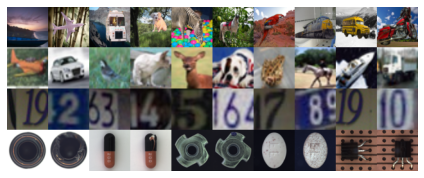
\includegraphics[width=\textwidth]{data/chapter_sgvaegan/all_grid.png}
    \caption{Examples of the datasets used in the experiments. Datasets from top row to bottom: COCOPlaces, CIFAR10, SVHN2 and MVTec-AD. MVTec-AD examples of normal and anomalous samples from the \textit{bottle, capsule, metal nut, pill}, and \textit{transistor} classes are shown.}
    \label{fig:all_grid}
\end{figure}

\subsection{Baseline methods}
We have selected unsupervised anomaly detectors mainly based on the review paper~\cite{vskvara2021comparison}, specifically those that were amongst the top performers on colored images. These models include:

\begin{description}
    \item[\textbf{Variational Autoencoder (VAE)}] - a convolutional VAE~\cite{an2015variational, kingma2013vae} that uses the sampled reconstruction error~\eqref{eq:rsscore}. The decoder variance $\sigma^2$ is estimated from the data.
    \item[\textbf{Feature-matching GAN (fmGAN)}] - a convolutional GAN model trained using the feature-matching loss~\cite{salimans2016fmgan}, similar to~\eqref{eq:recloss}. The anomaly score is based on the discriminator~\eqref{eq:discscore}.
    \item[\textbf{VAEGAN}] - a  convolutional VAE where reconstruction is enforced through a discriminator~\cite{larsen2016autoencoding}. The anomaly score is~\eqref{eq:discscore}.
    \item[\textbf{Deep Support Vector Data Description (DSVDD)}] - is a model~\cite{ruff2018deep} that learns a transformation of data via a neural network to a subspace where the anomalies lie outside of a hypersphere composed of transformed normal data. The anomaly score is then the distance of a point from the center of the hypersphere.
    \item[\textbf{fast Anomaly GAN (fAnoGAN)}] - a GAN model~\cite{schleglFAnoGANFastUnsupervised2019} trained via Wasserstein loss and gradient penalization that identifies anomalies by backward-searching the latent code $z$ that is the most likely to generate the given test samples.
    \item[\textbf{Counterfactual Generative Network (CGN)}] - this is a baseline model~\cite{sauer2021counterfactual} for the decomposition of data into three components. Although not originally intended as an anomaly detector, it can be used as one as it provides the discriminator score~\eqref{eq:discscore} and proved itself to be competitive in our experiments.
    \item[\textbf{Shape Guided VAE (SGVAE)}] - this is a modification of the proposed model that is trained without a discriminator and the reconstruction loss is $L_{\text{fm}}(x,0) = -\mathbb{E}_{q_{\phi}(z \vert x)}[\log p_{\theta}(x \vert z)]$, similar to a classical VAE. The anomaly score for this model is the sampled reconstruction error~\eqref{eq:rsscore}.
    \item[\textbf{Shape Guided VAEGAN (SGVAEGAN)}] - this is the basic proposed model that is trained in a completely unsupervised fashion without considering the full anomaly scores~\eqref{eq:totalscorejacobian},\eqref{eq:totalscoredisc}. Instead, the default anomaly score is the discriminator one~\eqref{eq:discscore}.
    \item[\textbf{SGVAE$_{\alpha}$}] - this is the SGVAE model where the score~\eqref{eq:totalscorejacobian} is considered. To compute the anomaly scores,  SGVAE models pre-trained in an unsupervised fashion were used and only the weights $\alpha$ were computed on a validation dataset.
    \item[\textbf{SGVAEGAN$_{\alpha}$}] - this is the full proposed model. In the first experiments, the score~\eqref{eq:totalscorejacobian} with the jacobian term was used, but later the jacobian score is dropped and the score~\eqref{eq:totalscoredisc} was computed instead, see the discussion in Sec.~\ref{sec:jacobian_contribution}.
\end{description}

The comparison of the baselines and the proposed models was conducted in a rigorous manner in accord with the extensive overview~\cite{vskvara2021comparison}. The datasets were split into training, validation, and test subsets for each of their classes (or subproblems in the case of the MVTec-AD dataset). Details on the splits for individual experiments can be found in the respective sections below. Then, for each such split and each model, 50 hyperparameter settings were randomly sampled from a set of possible values. The use of Bayesian optimization to select hyperparameters was considered but eventually dropped as it did not have an impact on the relative rank of the methods~\cite{vskvara2021comparison}. The individual models were trained using these hyperparameters. The validation set was used to select the best hyperparameter values for a given model on a specific subproblem. Unless mentioned otherwise, the experiments below report (ROC)AUC values of the selected models computed on the test set. The models were trained for 50 epochs each. All the models were implemented either in PyTorch or in Julia. The code for the proposed model can be found at \texttt{github.com/vitskvara/sgad} and the evaluation framework is at \texttt{github.com/vitskvara/GenerativeAD.jl}. 

\subsection{The contribution of the jacobian} \label{sec:jacobian_contribution}
\begin{table}[h] 
 \center 
 \begin{tabular}{c c c c c } 
 \toprule 
  class & AUC - no $J_d(x)$ & AUC - with $J_d(x)$ & $\alpha_r$ & $\alpha_j$  \\ 
  \midrule
  0 & 0.70 $\pm $0.04 & 0.70 $\pm $0.05 & 1.00 & 0.00  \\ 
  1 & 0.82 $\pm $0.01 & 0.82 $\pm $0.02 & 1.09 & -0.03  \\ 
  2 & 0.71 $\pm $0.02 & 0.72 $\pm $0.02 & 0.93 & -0.01  \\ 
  3 & 0.64 $\pm $0.02 & 0.64 $\pm $0.02 & 0.94 & 0.01  \\ 
  4 & 0.72 $\pm $0.03 & 0.72 $\pm $0.03 & 1.00 & 0.00  \\ 
  5 & 0.67 $\pm $0.01 & 0.66 $\pm $0.01 & 0.98 & 0.00  \\ 
  6 & 0.68 $\pm $0.02 & 0.68 $\pm $0.02 & 0.60 & 0.00  \\ 
  7 & 0.73 $\pm $0.05 & 0.73 $\pm $0.05 & 1.00 & 0.00  \\ 
  8 & 0.69 $\pm $0.04 & 0.71 $\pm $0.02 & 0.98 & -0.04  \\ 
  9 & 0.63 $\pm $0.05 & 0.63 $\pm $0.04 & 0.80 & 0.00  \\ 
  \bottomrule
 \end{tabular}
 \caption{Experiment with $J_d(x)$ on a subset of the SVHN2 dataset. For each normal class, training and testing sets containing 750 normal and 150 anomalous samples were used. To obtain the presented statistic, the subsets were sampled 5 times. The mean values of estimated $alpha$ weights are also presented and show that the weight of the jacobian term is suppressed during their computation.} 
 \label{tab:jacoceco_partial_experiment} 
\end{table}
We start the dissection of experimental results by an analysis of the jacobian term $J_d(x)$ in~\eqref{eq:totalscorejacobian}. See~Tab.~\ref{tab:jacoceco_partial_experiment} where the contribution of the term $J_d(x)$ to the anomaly score was measured by comparison of AUC performance of a model that used it and one that did not on a subset of the SVHN2 dataset. The difference in performance is almost negligible, but the computational costs of computing the jacobian matrix for image data are very high, making it extremely impractical. Therefore, the term is omitted from all further experiments, and the score~\eqref{eq:totalscoredisc} is used for the SGVAEGAN$_{\alpha}$ instead, while for SGVAE$_\alpha$, the term is dropped from~\eqref{eq:totalscorejacobian}.

\subsection{Detection of semantic anomalies} 
\begin{figure}[ht!]
    \centering
    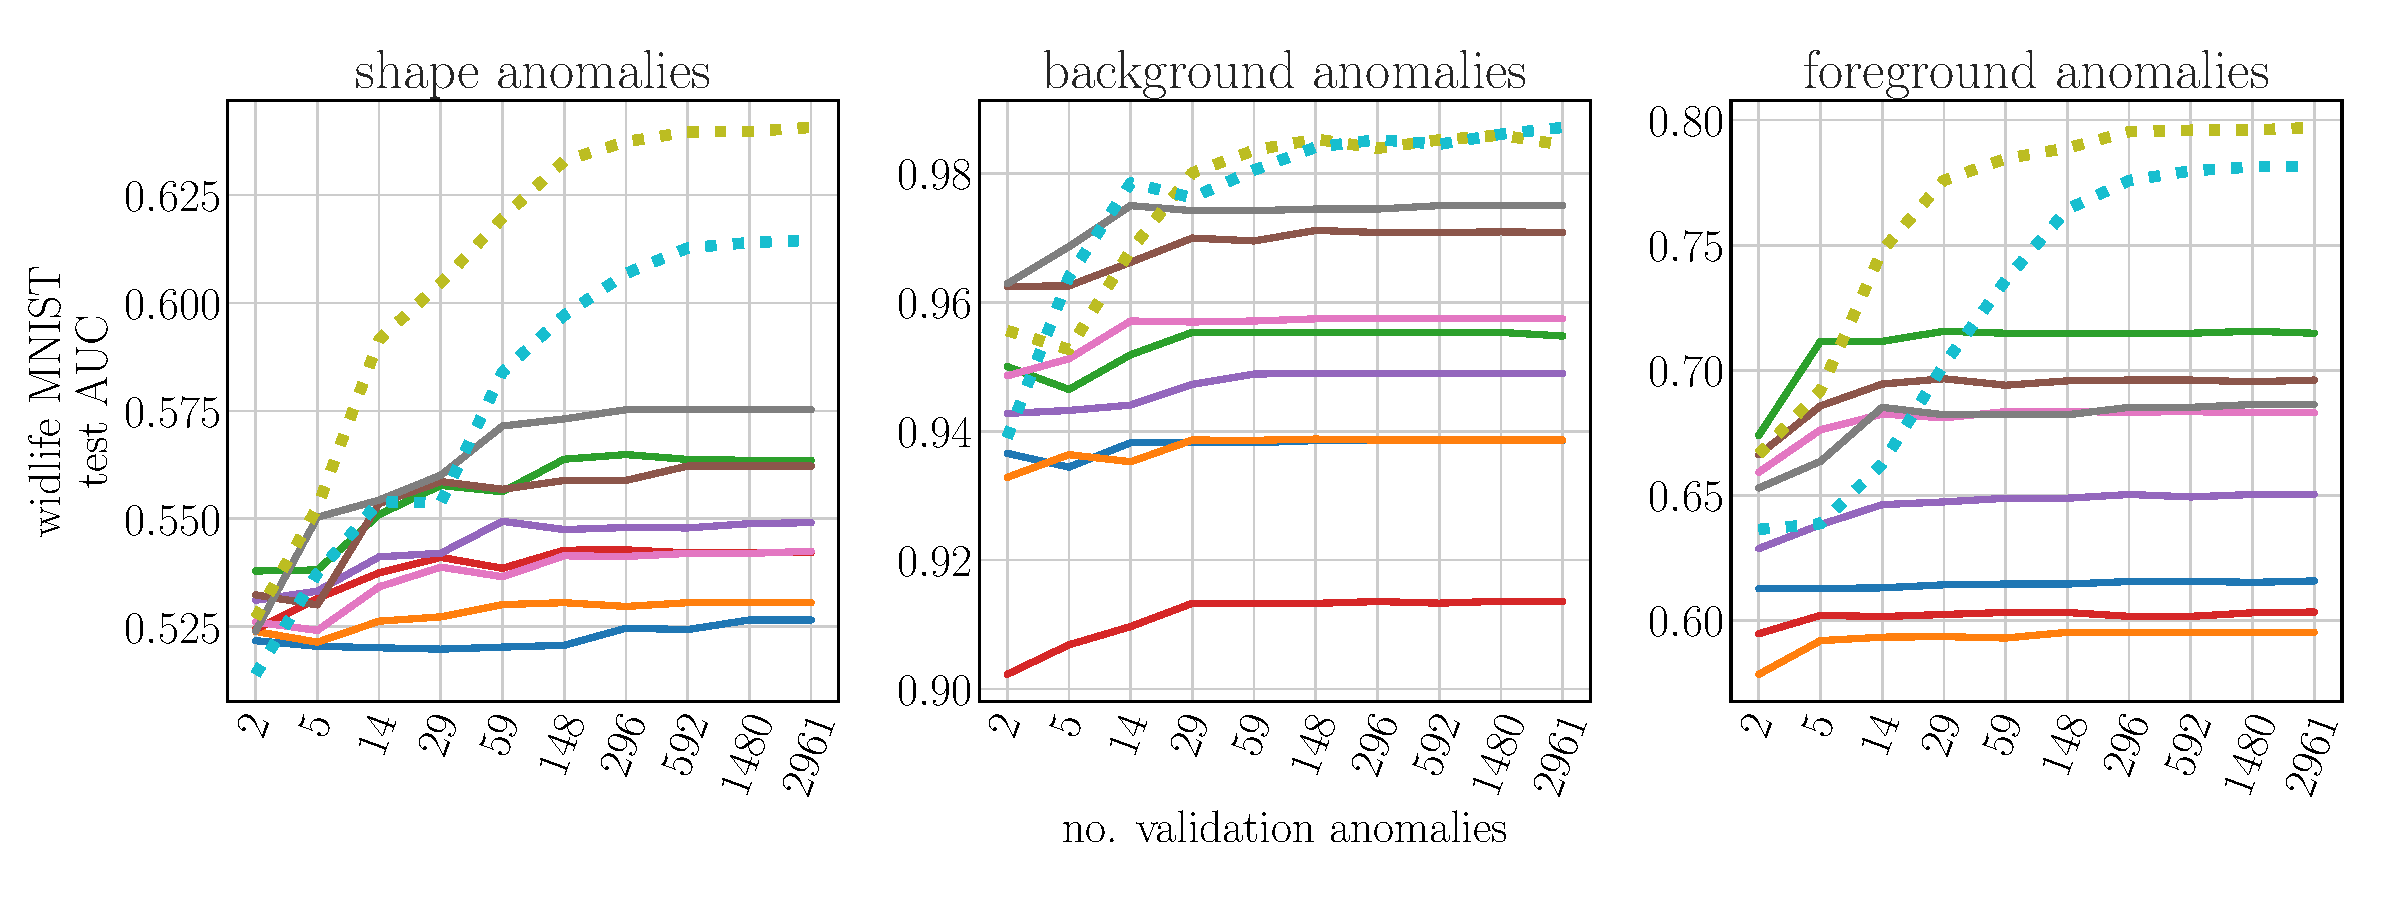
\includegraphics[width=\textwidth]{data/chapter_sgvaegan/multifactor_experiments_wmnist.pdf}
    
    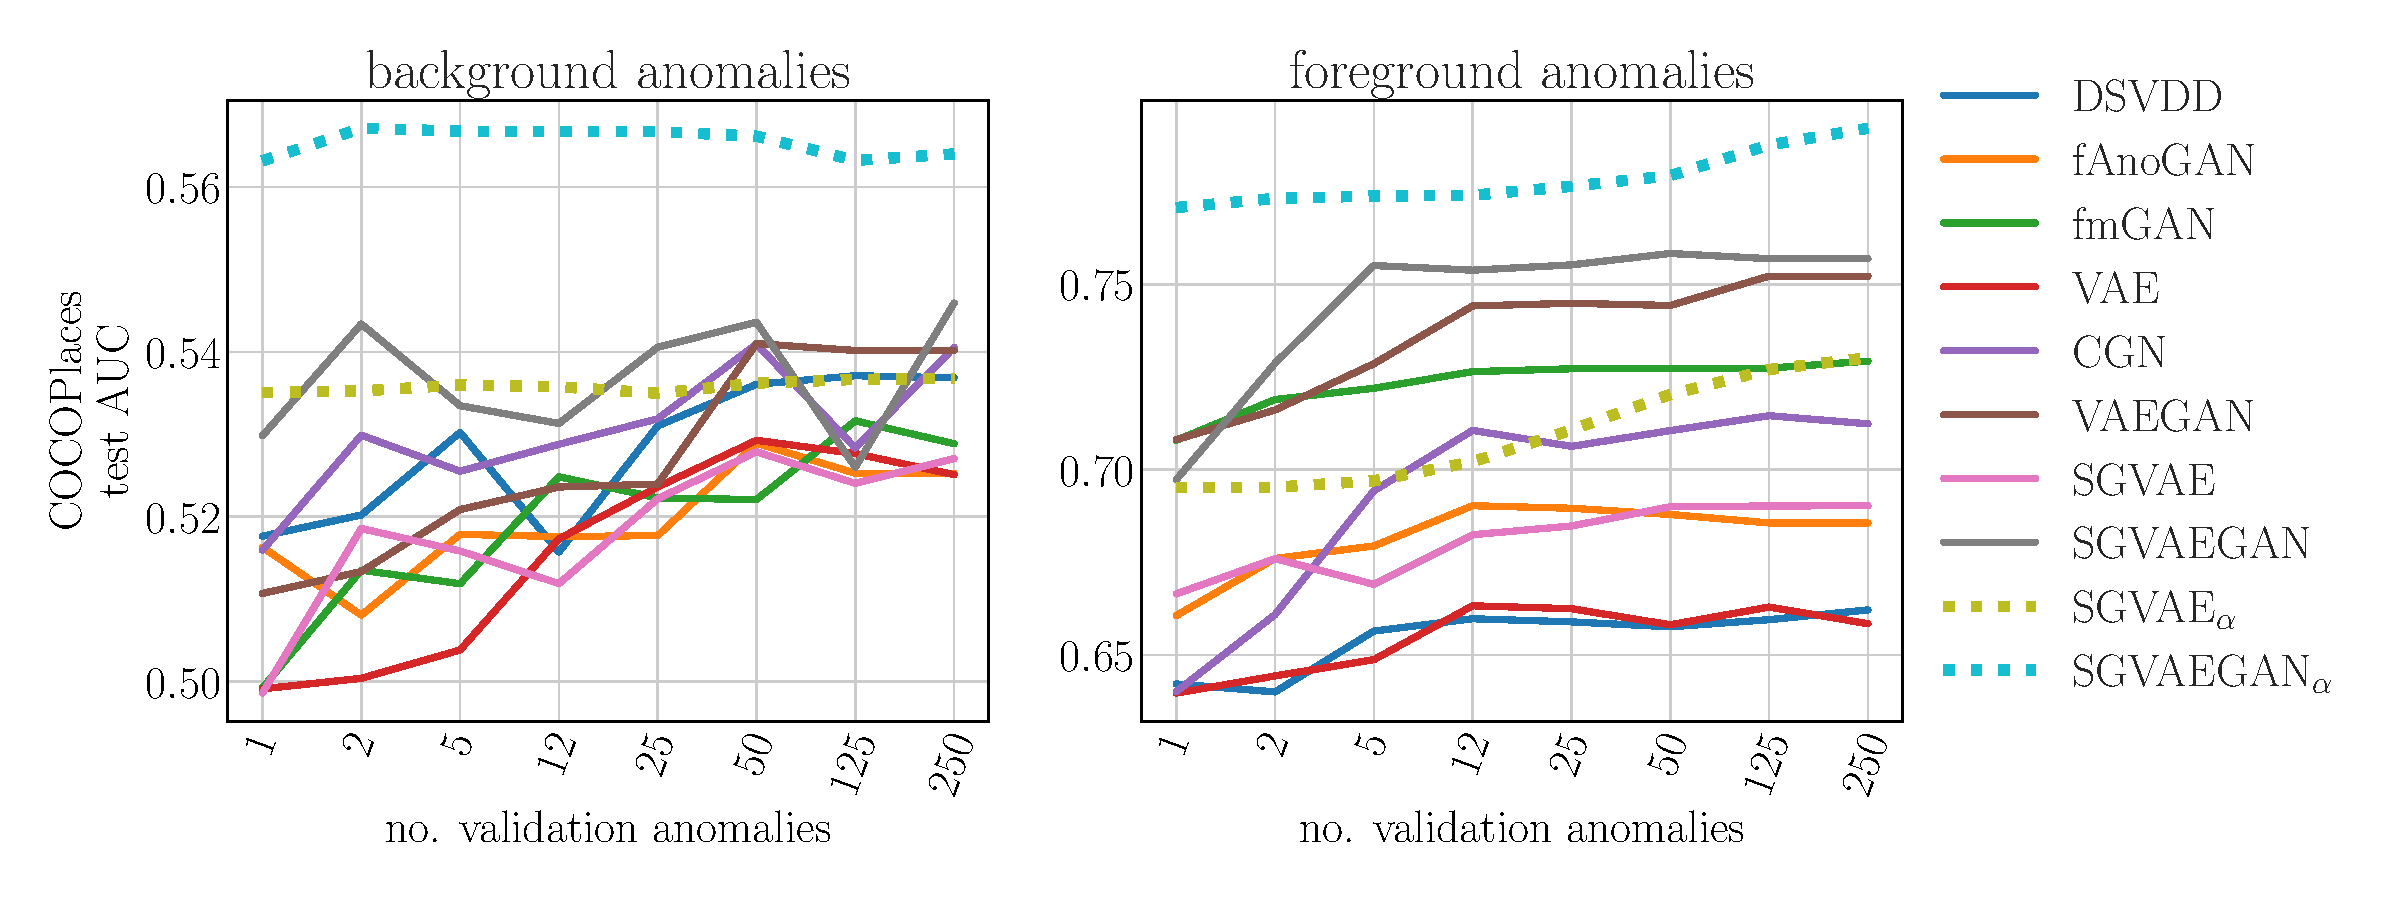
\includegraphics[width=\textwidth]{data/chapter_sgvaegan/multifactor_experiments_coco.pdf}
    \caption{Semantic anomaly detection experiment on the wildlife MNIST (top) and COCOPlaces (bottom) datasets. The x-axis covers a changing number of anomalies present in the validation dataset. The number of normal samples remains the same and is equal to the highest anomaly count presented in the figures. That means that in the most-informed scenario the validation set consists of the same number of anomalies and normal samples. The models are trained on the same training non-mixed data, their hyperparameters are selected on the validation dataset and the resulting test set AUC is reported on the y-axis. The AUC values are also averaged over 10 classes and a 5-fold random selection of the validation anomalies.}
    \label{fig:multifactor}
\end{figure}
In this experiment, we observe how the proposed detector behaves as it gradually incorporates more knowledge about labeled anomalies. To simulate a semantic anomaly scenario, the following training and testing protocol is observed on the Wildlife MNIST and COCOPlaces datasets. The training set consists of samples of one class (the whole experiment is repeated for all 10 classes) from the non-mixed version of the datasets (see Sec.~\ref{sec:datasets} for details of how this is generated). Then, for each factor of variation, validation and test sets are drawn from the mixed version of the dataset, where the anomality of a sample is based on whether the individual factor is the same or different as in the training dataset. We believe that this simulates a semantic anomaly problem, as for each factor, we have a validation/test dataset where there is data unseen by the model during training but not considered to be anomalous. 

See Fig.~\ref{fig:multifactor} for a comparison of the proposed models and the baselines. On wildlife MNIST, both of the proposed alternatives where the weights $\alpha$ are gradually improved with added anomalies outperform the remaining baselines convincingly in detection of all types of anomalous factors. On COCOPlaces, the difference is smaller and only the SGVAGEAN$_{\alpha}$ is clearly better. This stems from the dataset being much harder to correctly decompose. Unlike on wildlife MNIST, in some classes, there is no universal shape that all the objects share and the influence of the background is such that even for a human it is sometimes difficult to discern the principal object in an image. 

\subsection{Anomaly factor identification} \label{sec:anomaly_factor_identification}
It is possible to leverage the structure of the model presented above to identify the source of the anomality of an image through the information that is encoded in the individual latent spaces. The scenario here is that a potential anomaly has been identified, and now we want to know what is the cause of the anomaly. Under the formalism~\eqref{eq:pzy}, estimation of the anomaly factor  $p(y \vert z)\propto p(z \vert y)$ is possible only for proper distributions. Since we have opted for improper distribution to minimize the number of unknown parameters, we have to design an approximate method that does not rely on the availability of proper normalization. We propose two different approaches to it.

\textbf{Ranked detection}: we assume that the anomalous factor can be detected through the latent space kNN scores (\ref{eq:knnscore}). If only one factor is anomalous, then there should be a difference in the encodings of normal samples and the encodings of the anomalous one, and this difference should be visible in one of the latent spaces. In order to achieve this, the encodings of a sample $x$ for each latent space are computed. Then, kNN scores of these encodings with respect to encodings of normal data are computed, resulting in a vector of kNN scores $s_{\text{kNN}}(x) = (s_m(x), s_f(x), s_b(x))$. If the distances in the latent spaces were normalized, one could select the source of anomality (shape, background, or foreground texture) to have the highest kNN score. This is, however, not the case, even though all the latent spaces are regularized to resemble the same prior, see Fig.~\ref{fig:latent_decomposition_example}. Standardizing  the scores post-hoc to zero mean and unit variance did also not prove to work. Instead, for each individual latent space, we estimate the quantile of the sample using the rank of the kNN score of the tested sample among the kNN scores of normal data and compute its percentile -- the higher it is, the more anomalous the sample is in this latent space (at least with regard to the normal data). The latent space with the highest percentile should then be the source of the anomaly. The results for this method for models trained on the mixed version of the wildlife MNIST dataset (for a detailed description of the data see Sec.~\ref{sec:datasets}) are shown in~Tab.~\ref{tab:factor_detection}. 

\begin{table}[h] 
 \center 
 \begin{tabular}{c | c c c | c c}
 \toprule
 & \multicolumn{3}{c|}{ranked} & \multicolumn{2}{c}{masked} \\
  normal class & shape & background & foreground & background & foreground  \\ 
  \midrule 
  0 & 0.82 & 0.19 & 0.62 & 0.88 & 0.95  \\ 
  1 & 0.84 & 0.92 & 0.19 & 0.85 & 1.0  \\ 
  2 & 0.92 & 0.37 & 0.7 & 0.95 & 0.6  \\  
  3 & 0.55 & 0.86 & 0.24 & 0.63 & 0.96  \\
  4 & 0.79 & 0.46 & 0.85 & 0.62 & 1.0  \\ 
  5 & 0.57 & 0.89 & 0.31 & 0.72 & 1.0  \\ 
  6 & 0.74 & 0.95 & 0.52 & 0.96 & 0.96  \\
  7 & 0.47 & 0.84 & 0.75 & 0.87 & 0.98  \\
  8 & 0.64 & 0.64 & 0.62 & 0.98 & 0.97  \\
  9 & 0.88 & 0.27 & 0.1 & 0.77 & 0.94  \\
   \bottomrule
 \end{tabular}
 \caption{Accuracy of factor detection on the wildlife MNIST dataset for \textit{ranked} and \textit{masked} methods.} 
 \label{tab:factor_detection} 
\end{table}

\begin{figure}
    \centering
    \begin{center}
\begin{tikzpicture}
  \node[inner sep=0pt, label={\small train}] (train) at (-1.5,1.2) {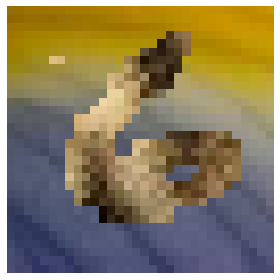
\includegraphics[scale=0.1]{data/chapter_sgvaegan/masked_examples/train_x.png}};

  % background anomaly
  \node[inner sep=0pt, label={\small $x_1$}]  at (0.6,1.9) {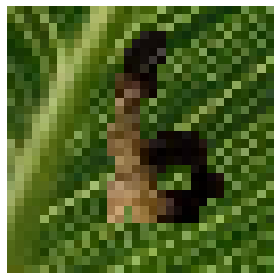
\includegraphics[scale=0.1]{data/chapter_sgvaegan/masked_examples/background_x.png}};
  \node[inner sep=0pt, label={\small $x_{r,1}$}] at (0.6,0.5) {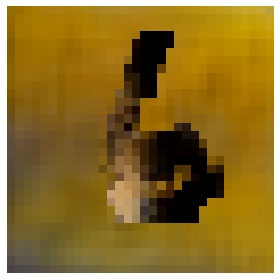
\includegraphics[scale=0.1]{data/chapter_sgvaegan/masked_examples/background_rx.png}};

  \node[inner sep=0pt, label={\small $m_1$}]  at (1.7,1.2) {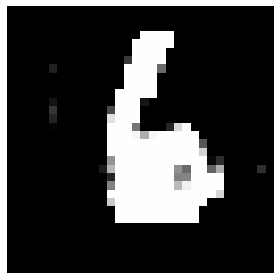
\includegraphics[scale=0.1]{data/chapter_sgvaegan/masked_examples/background_mask.png}};
  
  \node[inner sep=0pt, label={\small $bm_1$}]  at (2.8,1.9) {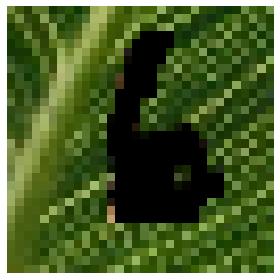
\includegraphics[scale=0.1]{data/chapter_sgvaegan/masked_examples/background_x_bg.png}};
  \node[inner sep=0pt, label={\small 0.23}] at (2.8,0.5) {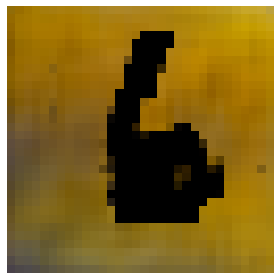
\includegraphics[scale=0.1]{data/chapter_sgvaegan/masked_examples/background_rx_bg.png}};
  
  \node[inner sep=0pt, label={\small $fm_1$}]  at (3.9,1.9) {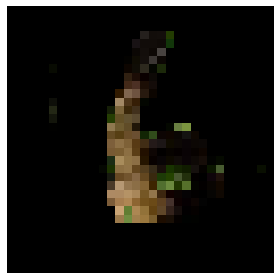
\includegraphics[scale=0.1]{data/chapter_sgvaegan/masked_examples/background_x_fg.png}};
  \node[inner sep=0pt, label={\small 0.05}] at (3.9,0.5) {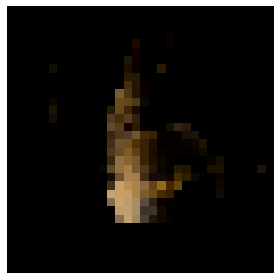
\includegraphics[scale=0.1]{data/chapter_sgvaegan/masked_examples/background_rx_fg.png}};

  % foreground anomaly
  \node[inner sep=0pt, label={\small $x_2$}]  at (6.0,1.9) {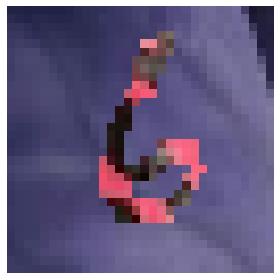
\includegraphics[scale=0.1]{data/chapter_sgvaegan/masked_examples/foreground_x.png}};
  \node[inner sep=0pt, label={\small $x_{r,2}$}] at (6.0,0.5) {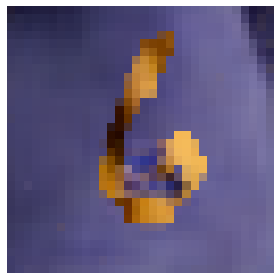
\includegraphics[scale=0.1]{data/chapter_sgvaegan/masked_examples/foreground_rx.png}};

  \node[inner sep=0pt, label={\small $m_2$}]  at (7.1,1.2) {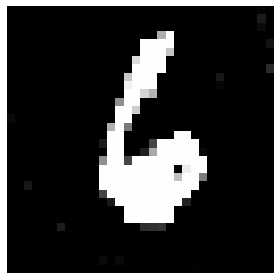
\includegraphics[scale=0.1]{data/chapter_sgvaegan/masked_examples/foreground_mask.png}};
  
  \node[inner sep=0pt, label={\small $bm_2$}]  at (8.2,1.9) {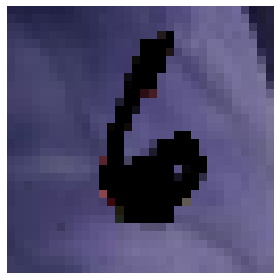
\includegraphics[scale=0.1]{data/chapter_sgvaegan/masked_examples/foreground_x_bg.png}};
  \node[inner sep=0pt, label={\small0.01}] at (8.2,0.5) {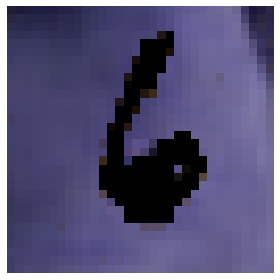
\includegraphics[scale=0.1]{data/chapter_sgvaegan/masked_examples/foreground_rx_bg.png}};
  
  \node[inner sep=0pt, label={\small $fm_1$}]  at (9.3,1.9) {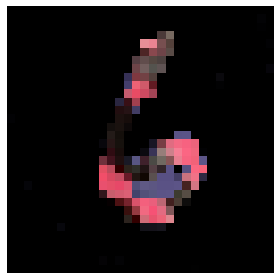
\includegraphics[scale=0.1]{data/chapter_sgvaegan/masked_examples/foreground_x_fg.png}};
  \node[inner sep=0pt, label={\small 0.18}] at (9.3,0.5) {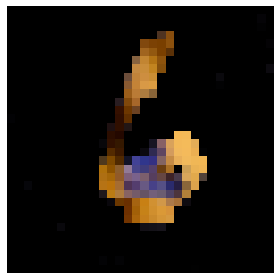
\includegraphics[scale=0.1]{data/chapter_sgvaegan/masked_examples/foreground_rx_fg.png}};
\end{tikzpicture}
\end{center}

    \caption{Masked detection technique for identifying the source of anomality. The model was originally trained on samples similar to the one on the very left, brown-striped sixes on purple-yellow background. To distinguish between anomalies in the background and foreground texture, a reconstruction $x_r$ and a mask $m$ are computed for a test sample $x_1$, which is anomalous in the background, and $x_2$, which is anomalous in the foreground texture. The scores $S_b$ \eqref{eq:sb}, $S_f$ \eqref{eq:sf} are computed as scaled differences between the original and reconstructed masked--out backgrounds, $b_m = x \odot (1-x_m)$ and foregrounds $f_m = x \odot x_m$ and their values are displayed between the image of the original and reconstructed foregrounds and backgrounds.}
    \label{fig:masked_detection}
\end{figure}

\textbf{Masked detection}: it is evident from the results of the ranked method that in some cases, it is difficult to find a model that would identify all three factors satisfactorily (better than random chance, which would give an accuracy score of 0.33). We believe it is because of the innate dependence of the result on the correctness of the mask, which might be nonsensical if one of the factors was not seen in training data. Therefore, we have devised a second factor detection technique, which only distinguishes between an anomaly in the background and foreground texture. For an input $x$, the reconstructed image $x'$ and a mask $x_m$is computed. Using these, we compute a normalized reconstruction error on the background and foreground separately
\begin{align}
    S_b & = \frac{\sum_i \left( (x_i-x_{i}') (1-x_{m,i}) \right) ^ 2}{\sum_i 1-x_{m,i}} \label{eq:sb} \\
    S_f & = \frac{\sum_i \left( (x_i-x_{i}') x_{m,i} \right) ^ 2}{\sum_i x_{m,i}}  \label{eq:sf}
\end{align}
where index $i$ goes over elements in all dimensions of an array $x \in \mathbb{R}^{h,w,3}$ representing an RGB image. See Fig.~\ref{fig:masked_detection} for an illustration of the principle of this method. The normalization factor is important since the object in the foreground usually covers fewer pixels than the background. If $S_b$ is higher, the prediction for the anomaly factor is "background" and vice versa. Results from the factor identification experiment using this method are in the second half of~Tab.~\ref{tab:factor_detection}. The background anomaly detection accuracies are not completely satisfactory on all digit classes. This is caused by some classes having very similar backgrounds, e.g. a very common misclassification for class "4" is that with anomalous background from classes "1" or "7", see~Fig.~\ref{fig:wmnist_grid}, where the background is reconstructed rather well, while even a small imprecision in the mask leads to a high reconstruction error on the foreground. Still, this method of detection of the source of anomality might be useful in some real-world problems, given we can train the model to produce correct masks. The main benefit of these methods is that they are completely unsupervised and at this moment, we are not aware of any other unsupervised anomaly detection method that would offer some kind of explainability of the source of anomality in image data.

\subsection{Anomaly detection on benchmark datasets} \label{sec:benchmarks}
\begin{figure}[ht!]
    \centering
        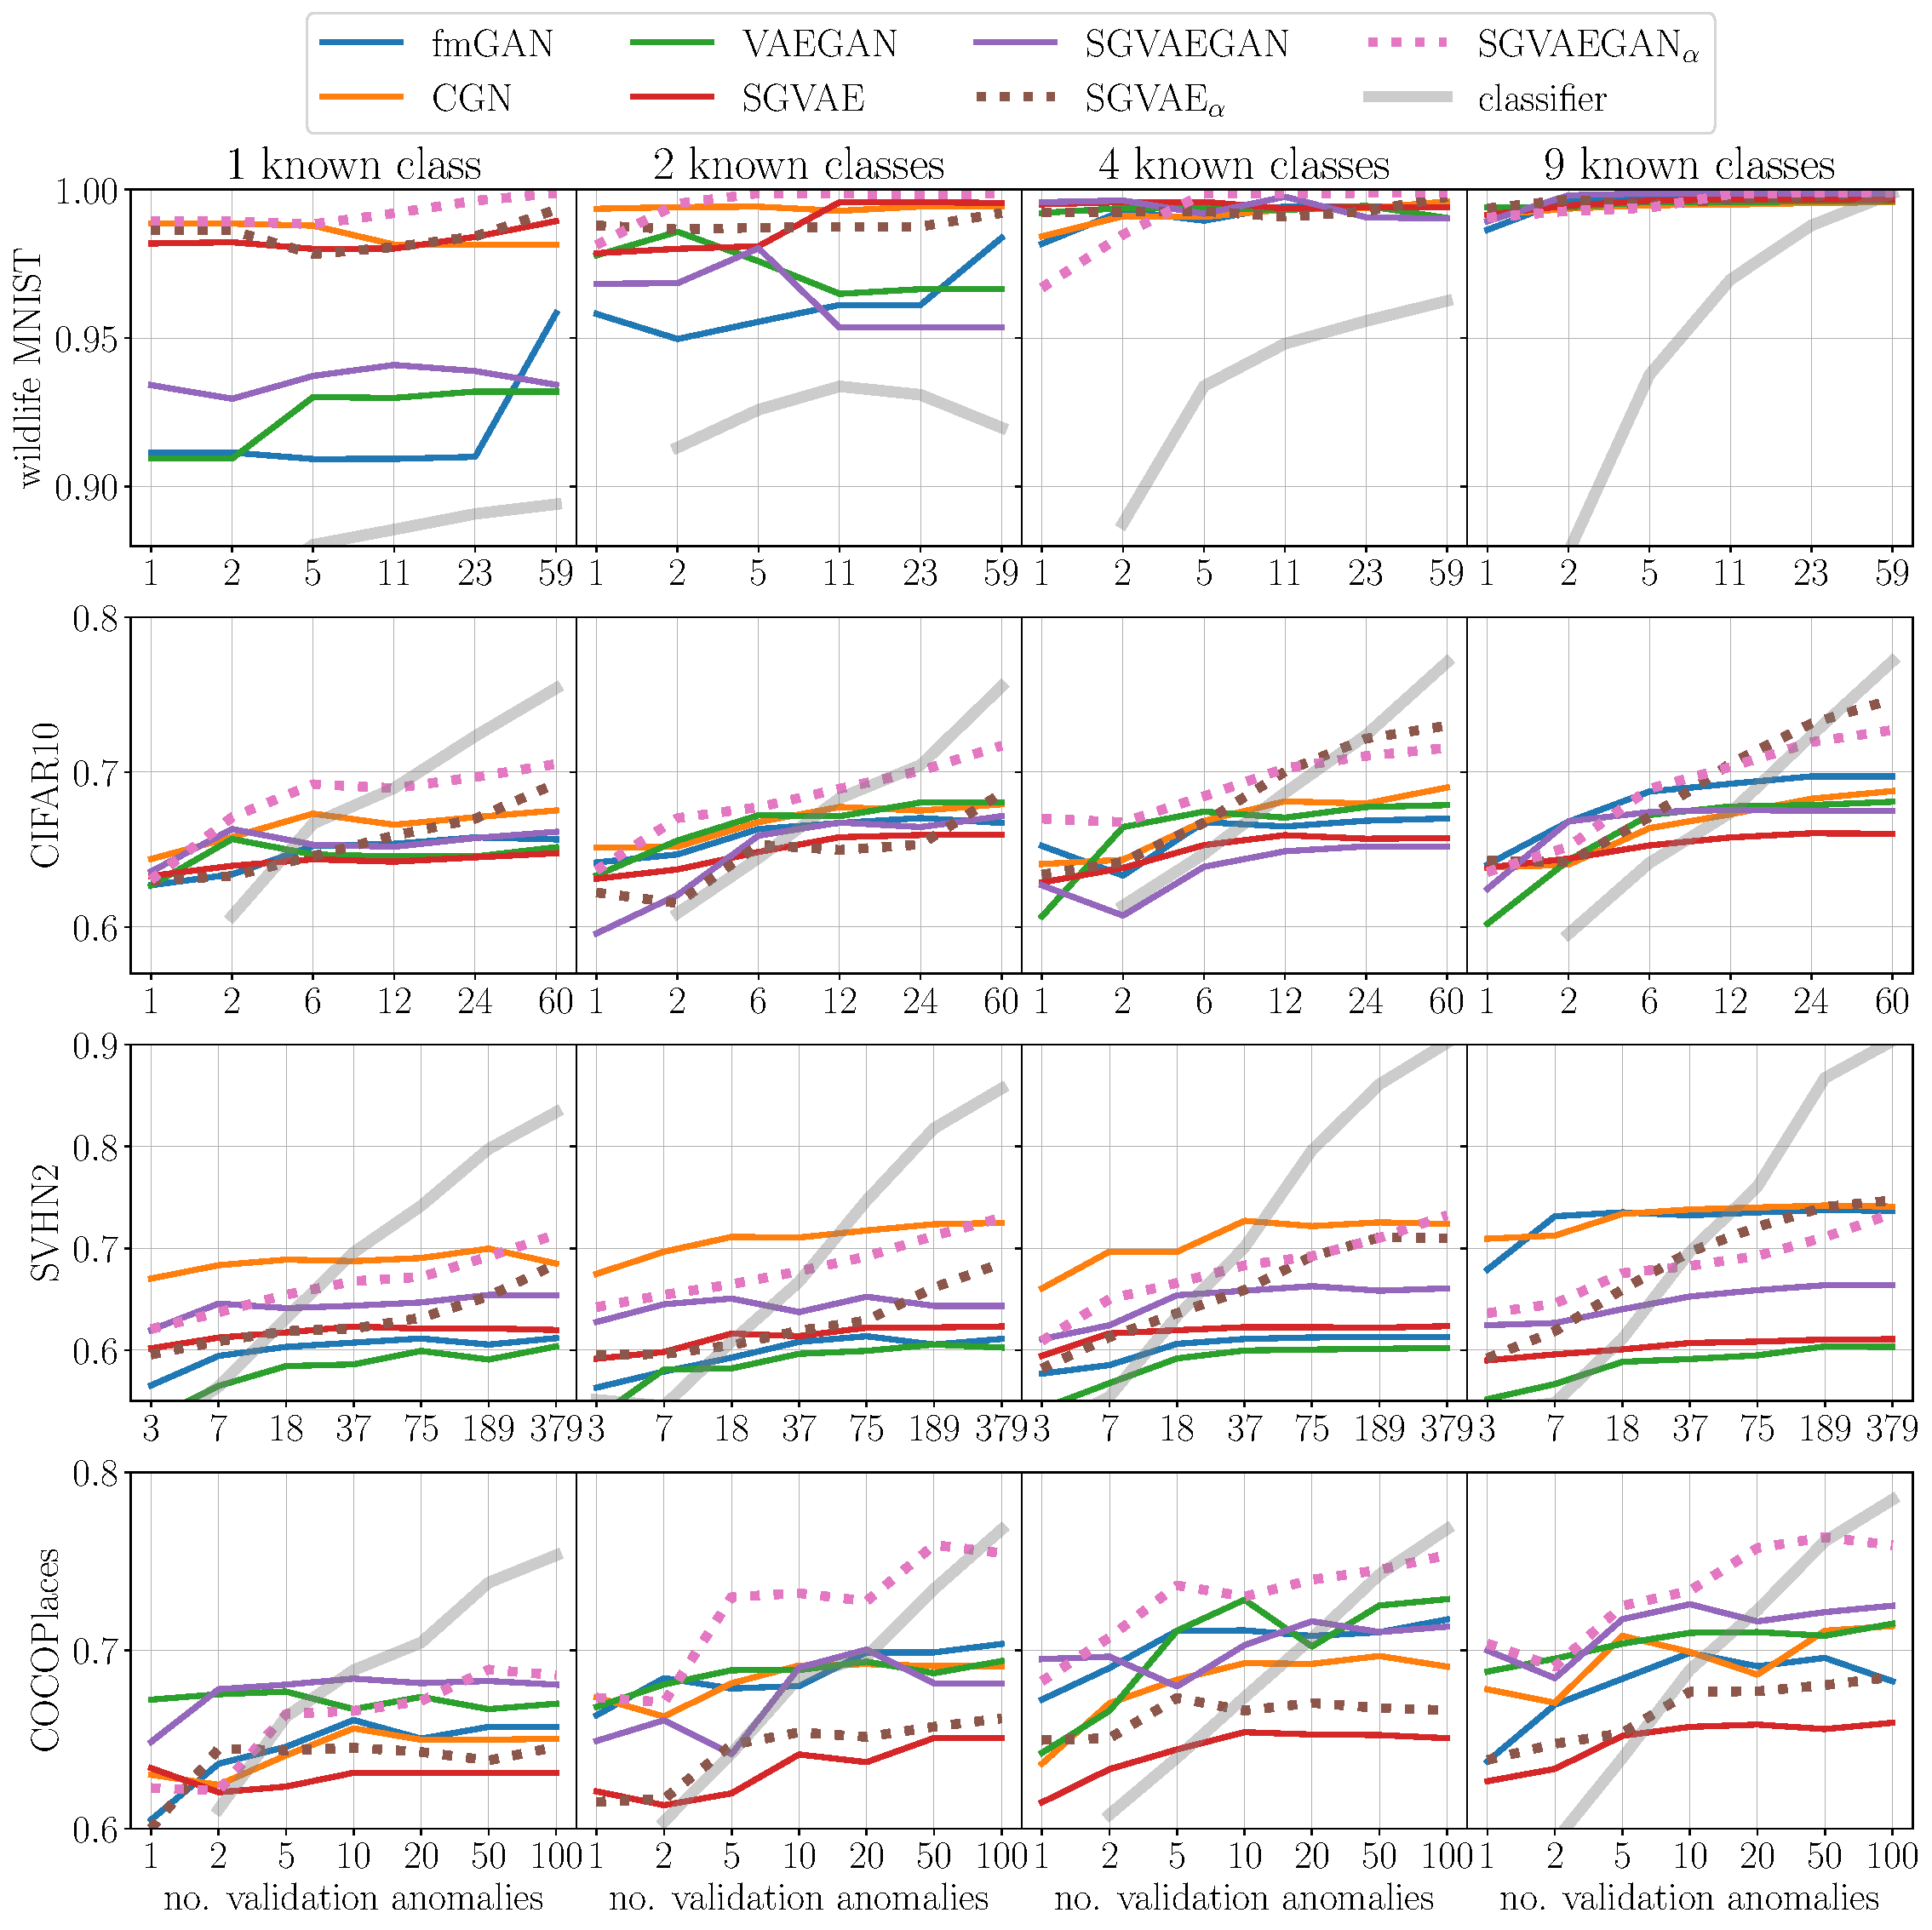
\includegraphics[width=\textwidth]{data/chapter_sgvaegan/all.pdf}
    \caption{Comparison of models on selected image datasets for the leave-one-in experiment. The x-axis covers a changing number of anomalies in the validation dataset, which is used for hyperparameter selection and $\alpha$ computation. The y-axis reports the average test AUC over 10 normal classes. The columns capture experiments with varying availability of validation samples from different anomalous classes, while anomalies of all classes are present in the test set. The number of normal samples in the validation set is the following: wildlife MNIST: 1184, CIFAR10: 1200, SVHN2: 3792, COCOPlaces: 100.}
    \label{fig:kplots}
\end{figure}

This experiment compares the proposed model in a traditional anomaly detection scenario on the datasets described in Sec.~\ref{sec:datasets}. We assume the leave-one-in scenario, which is that the training dataset contains samples from one class and the rest is considered to be anomalous in validation and test datasets. We believe this is a good representation of a semantic anomaly detection problem as well as being a more realistic option since in real-world problems, anomalies may come from many varying distributions. In this regard, we disagree with the authors of~\cite{ahmed2020detecting} which propose the alternative of leave-one-out, stating that in most anomaly detection problems, we want to detect only small perturbations from the target class. However, traditional image benchmarks don't allow for this anyway as the classes are very distinct even in the latter case. To really test models under this assumption, we have included the MVTec-AD dataset where the normal and anomalous data differ only in detail.

\begin{table}[ht!] 
 \center 
 \resizebox{\textwidth}{!}{ 
 \begin{tabular}{c c c c c c c c c c c } 
  problem & \rotatebox{90}{DSVDD} & \rotatebox{90}{fAnoGAN} & \rotatebox{90}{fmGAN} & \rotatebox{90}{VAE} & \rotatebox{90}{CGN} & \rotatebox{90}{VAEGAN} & \rotatebox{90}{SGVAE} & \rotatebox{90}{SGVAEGAN} & \rotatebox{90}{SGVAE$_{\alpha}$} & \rotatebox{90}{SGVAEGAN$_{\alpha}$}  \\ 
  \midrule 
  bottle & 0.81 & \cellcolor{gray!30} 0.97 & \cellcolor{gray!15} 0.95 & \cellcolor{gray!45} 0.98 & 0.90 & 0.85 & \cellcolor{gray!45} 0.98 & 0.83 & \cellcolor{gray!30} 0.97 & 0.92  \\ 
  capsule & 0.65 & 0.69 & 0.67 & \cellcolor{gray!15} 0.74 & 0.69 & 0.58 & \cellcolor{gray!30} 0.76 & 0.66 & \cellcolor{gray!45} 0.80 & 0.67  \\ 
  nut & 0.78 & 0.72 & \cellcolor{gray!45} 0.88 & 0.71 & 0.82 & \cellcolor{gray!15} 0.84 & 0.69 & 0.78 & 0.81 & \cellcolor{gray!30} 0.86  \\ 
  pill & 0.64 & 0.71 & \cellcolor{gray!15} 0.73 & \cellcolor{gray!15} 0.73 & 0.59 & 0.70 & \cellcolor{gray!30} 0.77 & 0.72 & \cellcolor{gray!45} 0.78 & \cellcolor{gray!15} 0.73  \\ 
  transistor & 0.69 & 0.77 & \cellcolor{gray!45} 0.90 & \cellcolor{gray!15} 0.81 & \cellcolor{gray!30} 0.88 & 0.75 & 0.78 & 0.79 & \cellcolor{gray!15} 0.81 & 0.79  \\ 
  \midrule
  mean rank & 8.90 & 6.20 & \cellcolor{gray!30} 3.50 & \cellcolor{gray!15} 4.20 & 5.50 & 7.60 & 4.50 & 7.00 & \cellcolor{gray!45} 2.80 & 4.80  \\ 
  \bottomrule
 \end{tabular}
 }
 \caption{Aggregated performance in test AUC of models on MVTec-AD problems.} 
 \label{tab:mvtec} 
\end{table}

To simulate a broader range of operating conditions, experiments with different anomalous classes in the validation set were conducted. For each normal class, samples from only a limited number of anomalous classes were sampled to the validation set, while the test set contained anomalies from all the classes left out from training. An example with 4 anomalous classes known in validation: training of models was done using class "1" of the SVHN2 dataset. The validation dataset contained normal data from class "1" and anomalies sampled from classes "2", "3", "4" and "5". The testing dataset contained normal samples from class "1" and anomalies sampled from all the remaining classes. This scenario is meant to test the robustness of methods to validation/test discrepancy which might occur in some real-world scenarios. The normal data split is 60/20/20\%, 50\% of available anomalies are in the test set and the number of validation anomalies is varied to obtain the x-axis in Fig.~\ref{fig:kplots}. This figure contains the overall comparison of a selection of the best-performing models to improve readability, a complete comparison of all baselines is e.g. in Tab.~\ref{tab:loi_ranks_per_ac}.

\begin{figure}[ht!] 
    \centering
    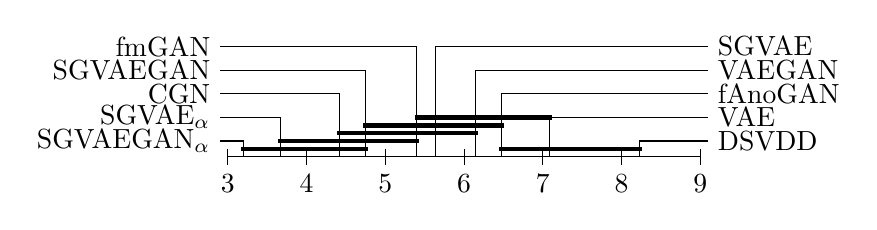
\begin{tikzpicture}[scale=1.0] 
  \draw (3.0,0) -- (9.0,0); 
  \foreach \x in {3,...,9} \draw (\x,0.10) -- (\x,-0.10) node[anchor=north]{$\x$}; 
  \draw (3.2,0) -- (3.2,0.19999999999999998) -- (2.9, 0.19999999999999998) node[anchor=east] {SGVAEGAN$_{\alpha}$}; 
  \draw (3.6625,0) -- (3.6625,0.5) -- (2.9, 0.5) node[anchor=east] {SGVAE$_{\alpha}$}; 
  \draw (4.4125,0) -- (4.4125,0.7999999999999999) -- (2.9, 0.7999999999999999) node[anchor=east] {CGN}; 
  \draw (4.75,0) -- (4.75,1.0999999999999999) -- (2.9, 1.0999999999999999) node[anchor=east] {SGVAEGAN}; 
  \draw (5.4,0) -- (5.4,1.4) -- (2.9, 1.4) node[anchor=east] {fmGAN}; 
  \draw (5.6375,0) -- (5.6375,1.4) -- (9.1, 1.4) node[anchor=west] {SGVAE}; 
  \draw (6.15,0) -- (6.15,1.0999999999999999) -- (9.1, 1.0999999999999999) node[anchor=west] {VAEGAN}; 
  \draw (6.475,0) -- (6.475,0.8) -- (9.1, 0.8) node[anchor=west] {fAnoGAN}; 
  \draw (7.0875,0) -- (7.0875,0.5) -- (9.1, 0.5) node[anchor=west] {VAE}; 
  \draw (8.225,0) -- (8.225,0.2) -- (9.1, 0.2) node[anchor=west] {DSVDD}; 
  \draw[line width=0.06cm,color=black,draw opacity=1.0] (3.170000047683716,0.1) -- (4.78,0.1); 
  \draw[line width=0.06cm,color=black,draw opacity=1.0] (3.6324999046325686,0.2) -- (5.430000095367432,0.2); 
  \draw[line width=0.06cm,color=black,draw opacity=1.0] (4.382499904632568,0.30000000000000004) -- (6.180000095367432,0.30000000000000004); 
  \draw[line width=0.06cm,color=black,draw opacity=1.0] (4.72,0.4) -- (6.504999904632569,0.4); 
  \draw[line width=0.06cm,color=black,draw opacity=1.0] (5.370000095367431,0.5) -- (7.117500095367432,0.5); 
  \draw[line width=0.06cm,color=black,draw opacity=1.0] (6.444999904632568,0.1) -- (8.255000381469726,0.1); 
 \end{tikzpicture} 

    \caption{A critical difference diagram that shows mean ranks of models from Tab.~\ref{tab:loi_ranks_per_ac}. The difference in the performance of 2 models compared on 40 datasets to be statistically significant on level 10\% must be greater than the value of the Nemenyi test $CD_{0.1}$=1.95. The thick horizontal lines connect the models with performance differences less than this.}
    \label{fig:cd}
\end{figure}

Apart from the SVHN2 dataset, the proposed model outperforms the baselines after already seeing some 10 examples of anomalies, in some cases even less. This is also documented in Tab.~\ref{tab:loi_ranks_per_ac} which contains a more detailed comparison of all baselines in the case of 2\% of labeled anomalies from 4 classes in the validation dataset. The proposed method is also relatively robust to the validation/test anomaly distribution discrepancy. This means that the tuning of the $\alpha$ coefficients focuses on identifying the normal class as well as on the detection of seen anomalies. See Tab.~\ref{tab:mvtec} for the results on the MVTec-AD subproblems. Here the alternative SGVAE$_{\alpha}$ trained without a discriminator performs better. A summary comparison of baselines is also presented in the critical difference diagram in Fig.~\ref{fig:cd}, where mean ranks of models are compared using the methodology presented in~\cite{demsar2006statistical}. Of the top four models that are statistically indistinguishable, there are three that were proposed in this paper.

\begin{table}[ht!] 
 \center 
 \resizebox{\textwidth}{!}{ 
 \begin{tabular}{c c c c c c c c c c c c } 
  & class & \rotatebox{90}{DSVDD} & \rotatebox{90}{fAnoGAN} & \rotatebox{90}{fmGAN} & \rotatebox{90}{VAE} & \rotatebox{90}{CGN} & \rotatebox{90}{VAEGAN} & \rotatebox{90}{SGVAE} & \rotatebox{90}{SGVAEGAN} & \rotatebox{90}{SGVAE$_{\alpha}$} & \rotatebox{90}{SGVAEGAN$_{\alpha}$}  \\ 
  \toprule
  \parbox[t]{1mm}{\multirow{10}{*}{\rotatebox[origin=c]{90}{wildlife MNIST}}} & 0 & 0.82 & \cellcolor{gray!15} 0.98 & \cellcolor{gray!45} 1.00 & 0.94 & \cellcolor{gray!45} 1.00 & \cellcolor{gray!45} 1.00 & \cellcolor{gray!45} 1.00 & \cellcolor{gray!45} 1.00 & \cellcolor{gray!30} 0.99 & \cellcolor{gray!45} 1.00  \\ 
   & 1 & \cellcolor{gray!30} 0.88 & \cellcolor{gray!45} 1.00 & \cellcolor{gray!45} 1.00 & \cellcolor{gray!45} 1.00 & \cellcolor{gray!45} 1.00 & \cellcolor{gray!45} 1.00 & \cellcolor{gray!45} 1.00 & \cellcolor{gray!45} 1.00 & \cellcolor{gray!45} 1.00 & \cellcolor{gray!45} 1.00  \\ 
    & 2 & 0.63 & \cellcolor{gray!15} 0.97 & \cellcolor{gray!45} 1.00 & 0.85 & \cellcolor{gray!30} 0.99 & \cellcolor{gray!45} 1.00 & 0.96 & 0.93 & \cellcolor{gray!30} 0.99 & \cellcolor{gray!45} 1.00  \\ 
    & 3 & \cellcolor{gray!15} 0.83 & \cellcolor{gray!30} 0.99 & \cellcolor{gray!30} 0.99 & \cellcolor{gray!30} 0.99 & \cellcolor{gray!30} 0.99 & \cellcolor{gray!30} 0.99 & \cellcolor{gray!45} 1.00 & \cellcolor{gray!45} 1.00 & \cellcolor{gray!45} 1.00 & \cellcolor{gray!45} 1.00  \\ 
    & 4 & \cellcolor{gray!15} 0.91 & \cellcolor{gray!45} 1.00 & \cellcolor{gray!30} 0.99 & \cellcolor{gray!30} 0.99 & \cellcolor{gray!45} 1.00 & \cellcolor{gray!45} 1.00 & \cellcolor{gray!45} 1.00 & \cellcolor{gray!30} 0.99 & \cellcolor{gray!45} 1.00 & \cellcolor{gray!45} 1.00  \\ 
    & 5 & 0.39 & \cellcolor{gray!15} 0.93 & \cellcolor{gray!30} 0.99 & 0.85 & \cellcolor{gray!30} 0.99 & \cellcolor{gray!30} 0.99 & \cellcolor{gray!45} 1.00 & \cellcolor{gray!45} 1.00 & \cellcolor{gray!45} 1.00 & \cellcolor{gray!45} 1.00  \\ 
    & 6 & \cellcolor{gray!30} 0.69 & \cellcolor{gray!45} 1.00 & \cellcolor{gray!45} 1.00 & \cellcolor{gray!45} 1.00 & \cellcolor{gray!45} 1.00 & \cellcolor{gray!45} 1.00 & \cellcolor{gray!45} 1.00 & \cellcolor{gray!45} 1.00 & \cellcolor{gray!45} 1.00 & \cellcolor{gray!45} 1.00  \\ 
    & 7 & 0.92 & \cellcolor{gray!30} 0.99 & \cellcolor{gray!30} 0.99 & \cellcolor{gray!45} 1.00 & \cellcolor{gray!30} 0.99 & \cellcolor{gray!30} 0.99 & \cellcolor{gray!45} 1.00 & \cellcolor{gray!45} 1.00 & \cellcolor{gray!45} 1.00 & \cellcolor{gray!15} 0.97  \\ 
    & 8 & \cellcolor{gray!45} 1.00 & \cellcolor{gray!45} 1.00 & \cellcolor{gray!45} 1.00 & \cellcolor{gray!45} 1.00 & \cellcolor{gray!45} 1.00 & \cellcolor{gray!45} 1.00 & \cellcolor{gray!45} 1.00 & \cellcolor{gray!45} 1.00 & \cellcolor{gray!45} 1.00 & \cellcolor{gray!45} 1.00  \\ 
    & 9 & 0.71 & \cellcolor{gray!15} 0.94 & \cellcolor{gray!30} 0.99 & \cellcolor{gray!15} 0.94 & \cellcolor{gray!30} 0.99 & \cellcolor{gray!45} 1.00 & \cellcolor{gray!30} 0.99 & \cellcolor{gray!45} 1.00 & \cellcolor{gray!30} 0.99 & \cellcolor{gray!45} 1.00  \\ 
  \midrule
    \parbox[t]{1mm}{\multirow{10}{*}{\rotatebox[origin=c]{90}{CIFAR10}}} & airplane & 0.72 & 0.72 & 0.68 & 0.68 & 0.68 & \cellcolor{gray!15} 0.78 & \cellcolor{gray!15} 0.78 & 0.76 & \cellcolor{gray!30} 0.81 & \cellcolor{gray!45} 0.87  \\ 
    & automobile & 0.63 & 0.56 & 0.69 & 0.62 & \cellcolor{gray!45} 0.78 & \cellcolor{gray!15} 0.75 & 0.46 & \cellcolor{gray!30} 0.76 & 0.74 & \cellcolor{gray!45} 0.78  \\ 
    & bird & 0.67 & 0.67 & 0.60 & 0.66 & 0.60 & 0.56 & \cellcolor{gray!30} 0.70 & 0.47 & \cellcolor{gray!15} 0.68 & \cellcolor{gray!45} 0.72  \\ 
    & cat & 0.61 & 0.58 & 0.59 & 0.57 & \cellcolor{gray!15} 0.62 & 0.60 & 0.59 & 0.56 & \cellcolor{gray!45} 0.69 & \cellcolor{gray!30} 0.65  \\ 
    & deer & 0.71 & \cellcolor{gray!15} 0.75 & 0.65 & 0.74 & 0.66 & 0.63 & 0.74 & 0.66 & \cellcolor{gray!45} 0.78 & \cellcolor{gray!30} 0.77  \\ 
    & dog & 0.60 & 0.59 & \cellcolor{gray!15} 0.65 & 0.58 & 0.64 & 0.64 & 0.59 & 0.63 & \cellcolor{gray!30} 0.67 & \cellcolor{gray!45} 0.69  \\ 
    & frog & 0.71 & \cellcolor{gray!15} 0.76 & 0.71 & 0.75 & 0.67 & 0.69 & 0.73 & 0.60 & \cellcolor{gray!30} 0.78 & \cellcolor{gray!45} 0.82  \\ 
    & horse & 0.61 & 0.56 & 0.60 & 0.54 & \cellcolor{gray!45} 0.75 & \cellcolor{gray!30} 0.72 & 0.67 & 0.65 & \cellcolor{gray!15} 0.70 & 0.68  \\ 
    & ship & 0.74 & \cellcolor{gray!15} 0.80 & 0.77 & 0.71 & 0.74 & 0.71 & \cellcolor{gray!30} 0.82 & 0.72 & \cellcolor{gray!45} 0.84 & 0.79  \\ 
    & truck & 0.67 & 0.65 & \cellcolor{gray!45} 0.79 & 0.63 & \cellcolor{gray!15} 0.76 & 0.67 & 0.54 & 0.70 & 0.73 & \cellcolor{gray!30} 0.78  \\ 
    \midrule
    \parbox[t]{1mm}{\multirow{10}{*}{\rotatebox[origin=c]{90}{SVHN2}}} & 0 & 0.64 & 0.64 & 0.68 & 0.64 & \cellcolor{gray!45} 0.78 & 0.64 & 0.67 & 0.65 & \cellcolor{gray!15} 0.71 & \cellcolor{gray!30} 0.77  \\ 
    & 1 & 0.63 & 0.60 & 0.61 & 0.67 & \cellcolor{gray!15} 0.76 & 0.61 & 0.69 & 0.70 & \cellcolor{gray!30} 0.82 & \cellcolor{gray!45} 0.84  \\ 
    & 2 & 0.61 & 0.58 & 0.58 & 0.62 & \cellcolor{gray!45} 0.76 & 0.62 & 0.62 & 0.63 & \cellcolor{gray!30} 0.75 & \cellcolor{gray!15} 0.74  \\ 
    & 3 & 0.55 & 0.55 & 0.59 & 0.58 & \cellcolor{gray!45} 0.71 & 0.54 & 0.59 & \cellcolor{gray!15} 0.64 & \cellcolor{gray!15} 0.64 & \cellcolor{gray!30} 0.68  \\ 
    & 4 & 0.58 & 0.58 & 0.63 & 0.63 & \cellcolor{gray!45} 0.80 & 0.66 & 0.62 & 0.69 & \cellcolor{gray!15} 0.74 & \cellcolor{gray!30} 0.77  \\ 
    & 5 & 0.56 & 0.57 & 0.61 & 0.58 & \cellcolor{gray!45} 0.72 & 0.57 & 0.60 & 0.65 & \cellcolor{gray!15} 0.67 & \cellcolor{gray!30} 0.69  \\ 
    & 6 & 0.57 & 0.60 & 0.58 & 0.59 & \cellcolor{gray!45} 0.75 & 0.62 & 0.61 & 0.66 & \cellcolor{gray!30} 0.73 & \cellcolor{gray!15} 0.72  \\ 
    & 7 & 0.59 & 0.58 & 0.66 & 0.64 & \cellcolor{gray!45} 0.82 & 0.61 & 0.65 & 0.69 & \cellcolor{gray!15} 0.77 & \cellcolor{gray!30} 0.78  \\ 
    & 8 & 0.58 & 0.60 & 0.57 & 0.58 & \cellcolor{gray!30} 0.70 & 0.57 & 0.59 & \cellcolor{gray!15} 0.65 & \cellcolor{gray!15} 0.65 & \cellcolor{gray!45} 0.71  \\ 
    & 9 & 0.56 & 0.59 & 0.62 & 0.59 & \cellcolor{gray!45} 0.74 & 0.56 & 0.60 & 0.65 & \cellcolor{gray!15} 0.68 & \cellcolor{gray!30} 0.71  \\ 
    \midrule
    \parbox[t]{1mm}{\multirow{10}{*}{\rotatebox[origin=c]{90}{COCOPlaces}}} & airplane & 0.72 & 0.74 & \cellcolor{gray!15} 0.77 & 0.74 & 0.68 & \cellcolor{gray!30} 0.79 & 0.64 & \cellcolor{gray!45} 0.81 & \cellcolor{gray!15} 0.77 & \cellcolor{gray!45} 0.81  \\ 
    & bird & 0.48 & 0.48 & 0.64 & 0.53 & 0.64 & 0.61 & 0.47 & \cellcolor{gray!45} 0.69 & \cellcolor{gray!15} 0.66 & \cellcolor{gray!30} 0.68  \\ 
    & boat & 0.65 & 0.70 & \cellcolor{gray!45} 0.81 & \cellcolor{gray!15} 0.76 & \cellcolor{gray!15} 0.76 & \cellcolor{gray!30} 0.77 & \cellcolor{gray!30} 0.77 & 0.71 & \cellcolor{gray!30} 0.77 & \cellcolor{gray!45} 0.81  \\ 
    & bus & 0.58 & 0.82 & \cellcolor{gray!15} 0.85 & 0.67 & 0.83 & \cellcolor{gray!30} 0.87 & 0.74 & 0.70 & 0.78 & \cellcolor{gray!45} 0.89  \\ 
    & dog & \cellcolor{gray!30} 0.72 & \cellcolor{gray!15} 0.71 & \cellcolor{gray!15} 0.71 & \cellcolor{gray!30} 0.72 & 0.63 & 0.64 & \cellcolor{gray!15} 0.71 & 0.66 & \cellcolor{gray!15} 0.71 & \cellcolor{gray!45} 0.75  \\ 
    & horse & 0.58 & 0.57 & \cellcolor{gray!15} 0.69 & 0.65 & 0.59 & \cellcolor{gray!30} 0.71 & 0.65 & \cellcolor{gray!15} 0.69 & 0.64 & \cellcolor{gray!45} 0.74  \\ 
    & motorcycle & 0.63 & 0.65 & \cellcolor{gray!15} 0.75 & 0.60 & \cellcolor{gray!30} 0.77 & \cellcolor{gray!30} 0.77 & 0.69 & 0.73 & 0.66 & \cellcolor{gray!45} 0.78  \\ 
    & train & 0.64 & 0.71 & 0.68 & 0.65 & 0.55 & 0.62 & 0.69 & \cellcolor{gray!15} 0.74 & \cellcolor{gray!30} 0.75 & \cellcolor{gray!45} 0.77  \\ 
    & truck & 0.48 & 0.65 & 0.61 & 0.63 & 0.63 & \cellcolor{gray!30} 0.69 & 0.63 & \cellcolor{gray!45} 0.70 & \cellcolor{gray!15} 0.68 & 0.64  \\ 
    & zebra & 0.68 & 0.63 & 0.59 & 0.66 & \cellcolor{gray!30} 0.84 & \cellcolor{gray!15} 0.82 & 0.52 & 0.79 & \cellcolor{gray!45} 0.86 & \cellcolor{gray!30} 0.84  \\ 
  \midrule
  & mean rank & 8.23 & 6.48 & 5.40 & 7.09 & \cellcolor{gray!15} 4.41 & 6.15 & 5.64 & 4.75 & \cellcolor{gray!30} 3.66 & \cellcolor{gray!45} 3.20  \\ 
  \bottomrule
 \end{tabular}
 }
 \caption{Test AUC of models trained on the normal class marked in the first column of the table. The shading highlights the top 3 models. In this experiment, the validation dataset contained anomalies from 4 known classes, which is the same as the third column in Fig.~\ref{fig:kplots}. The ratio of normal data and anomalies in the validation dataset was 100:2. In absolute numbers, this means the following numbers of validation anomalies: wildlife MNIST: 23, CIFAR10: 24, SVHN2: 75, COCOPlaces: 2.} 
 \label{tab:loi_ranks_per_ac} 
\end{table}

If we assume that authors of other publications use default test/train splits and perform model hyperparameter selection on the same test set on which they report their results, the amount of labeled data that enters the model selection process is significant. Using the default splits on the SVHN2 dataset in the leave-one-in paradigm, the test set contains on average 2603 normal samples and 23429 anomalies (since the class distributions are unequal), while on CIFAR10 there are 900 normal and 9100 anomalous samples. Even if we consider the leave-one-out case, where the numbers of anomalies and normal data are switched, this is still a lot more labeled data than what we report e.g. in~Tab.~\ref{tab:loi_ranks_per_ac}. Also, by selecting the optimal model on the validation set and reporting on the test set, our experiments provide a fairer comparison of baselines.

A fully supervised classifier trained on the validation dataset is included in the comparison in Fig.~\ref{fig:kplots} as well to try to answer a question that is very pertinent for practitioners -- if you need at least some labeled anomalies to tune your unsupervised models anyway, what amount of labeled anomalies means that you can train a fully supervised classifier instead? Our comparison shows that this amount is surprisingly low, apart from the (relatively easy) wildlife MNIST dataset. This result is, of course, closely tied to the specific setting of our experiment and should not be extrapolated to other problems without further research.

% show identified anomalies
% show anomalies that are identified only after the alpha  tuning
% show the early stopping graphs?

\section{Conclusion}
We have defined a deep generative model for anomaly detection that uses several independent latent spaces to generate the data sample. The generative model is assumed to generate the normal class, and the flexibility of the latent spaces allows us to question which component of the test sample is anomalous. This concept has been applied to semantic anomaly detection of images for which we developed the SGVAEGAN model with independent latent spaces for shape, foreground, and background textures. The proposed model was tested on synthetic as well as real-world image datasets.

We have shown that the proposed model can detect the source of an anomaly in the sample on synthetic data. Another use of the separate scores is fine-tuning the anomaly score to the type of anomalies that are of interest. This has been achieved by learning the weights of the independent scores for known anomalies in the validation. The weights have been tuned to detect the known anomalies after seeing a few of their examples. Naturally, the performance of the proposed method improves with a growing number of available anomalies in the validation. However, the number of known anomalies is often low, since datasets with a high number of anomalies can be treated by supervised training. A comparison of the proposed method with a supervised classifier trained on the same amount of anomalies reveals that the supervised classifier outperforms any anomaly detector for a relatively low number of anomalous samples. This sets an upper bound on the meaningful range of problems suitable for anomaly detection methods. We recommend performing such an experiment for every anomaly detection method. 

The proposed SGVAEGAN model is a demonstration of the general approach, which can be used with any type of decomposition/disentanglement of the latent space. The requirement for the application of another generative model is that it has to be capable of learning the disentanglement in an unsupervised manner. Further research is required to find such a reliable model. 
